\chapter*{Oracle Apex}

\section{Langkah-Langkah membuat aplikasi menggunakan Apex}

Berikut langkah-langkah membuat aplikasi apex.
\begin{enumerate}
\item Buka website oracle apex dan klik sign in
\begin{figure}[H]
        \centerline{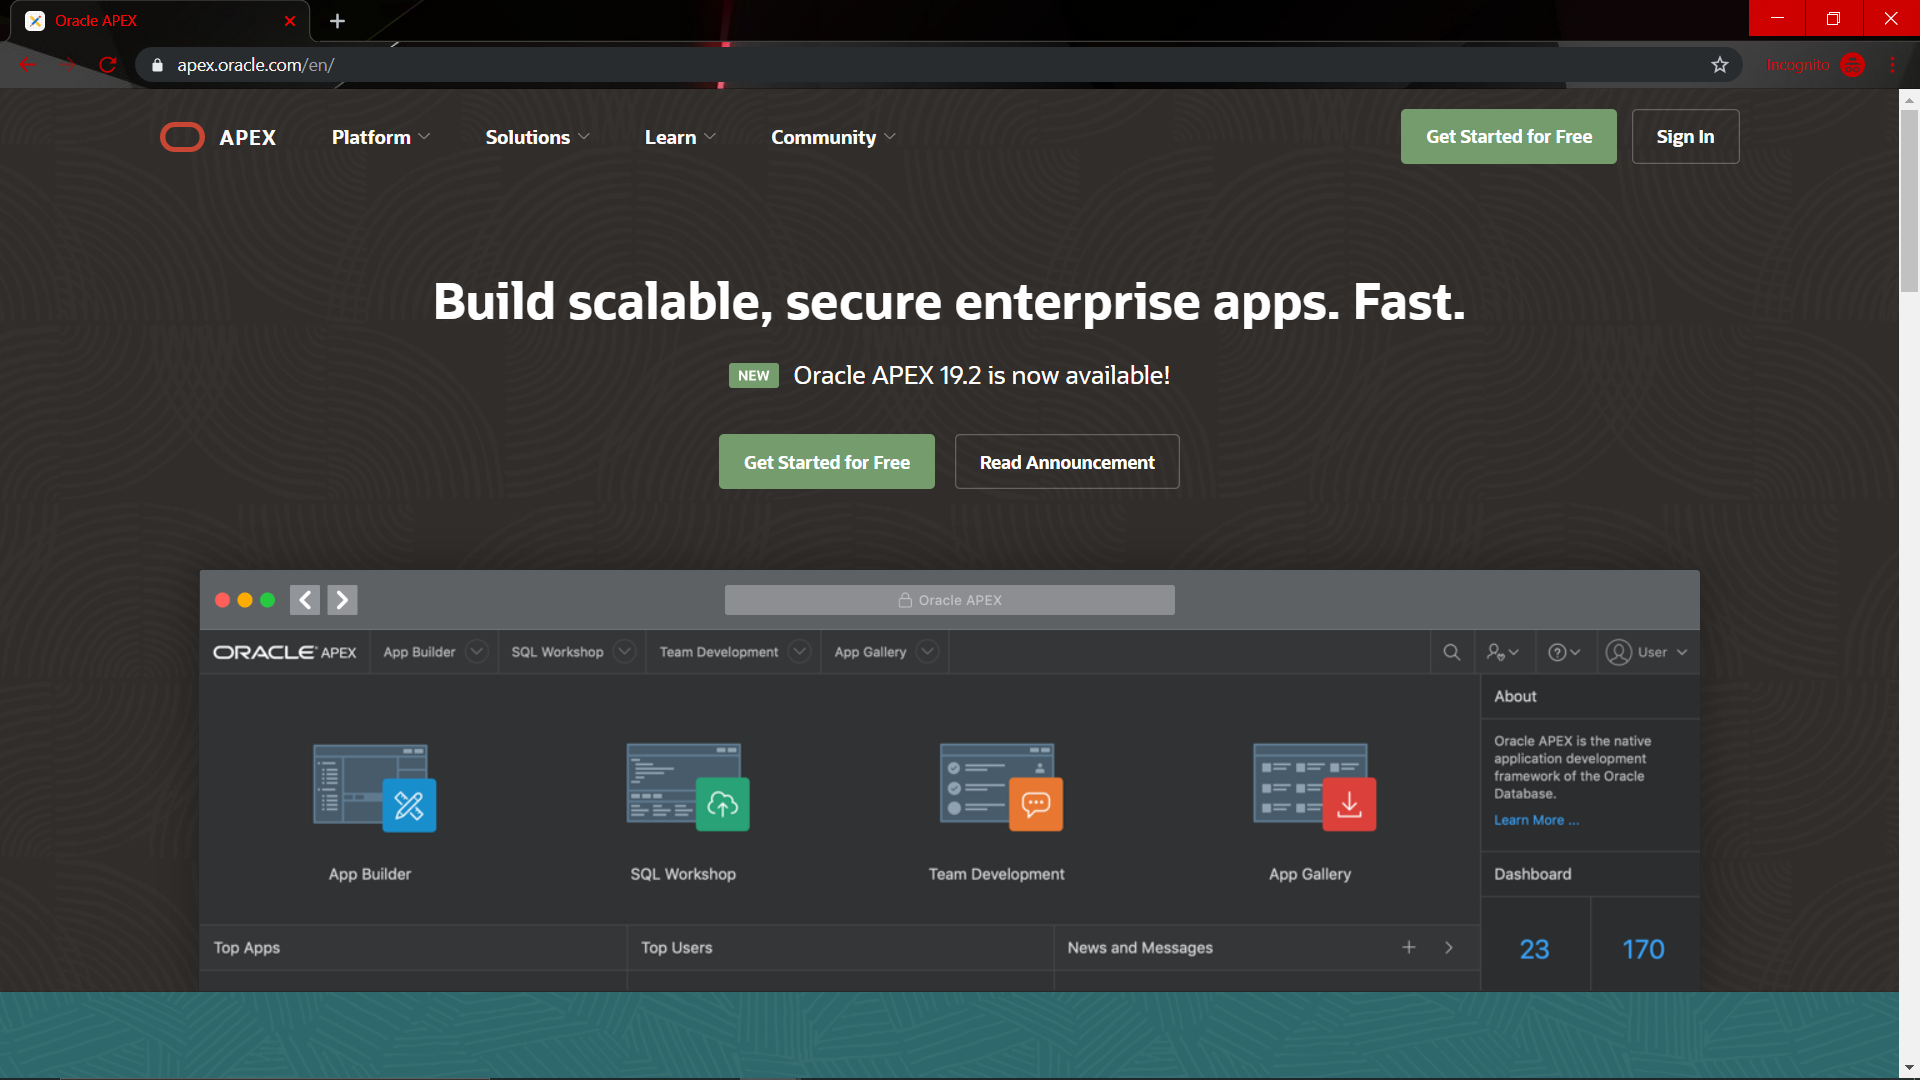
\includegraphics[scale=0.2]{figures/1}}
        \caption{Website}
		\label{langkah1}
\end{figure} \\

\item klik request workspace
\begin{figure}[H]
        \centerline{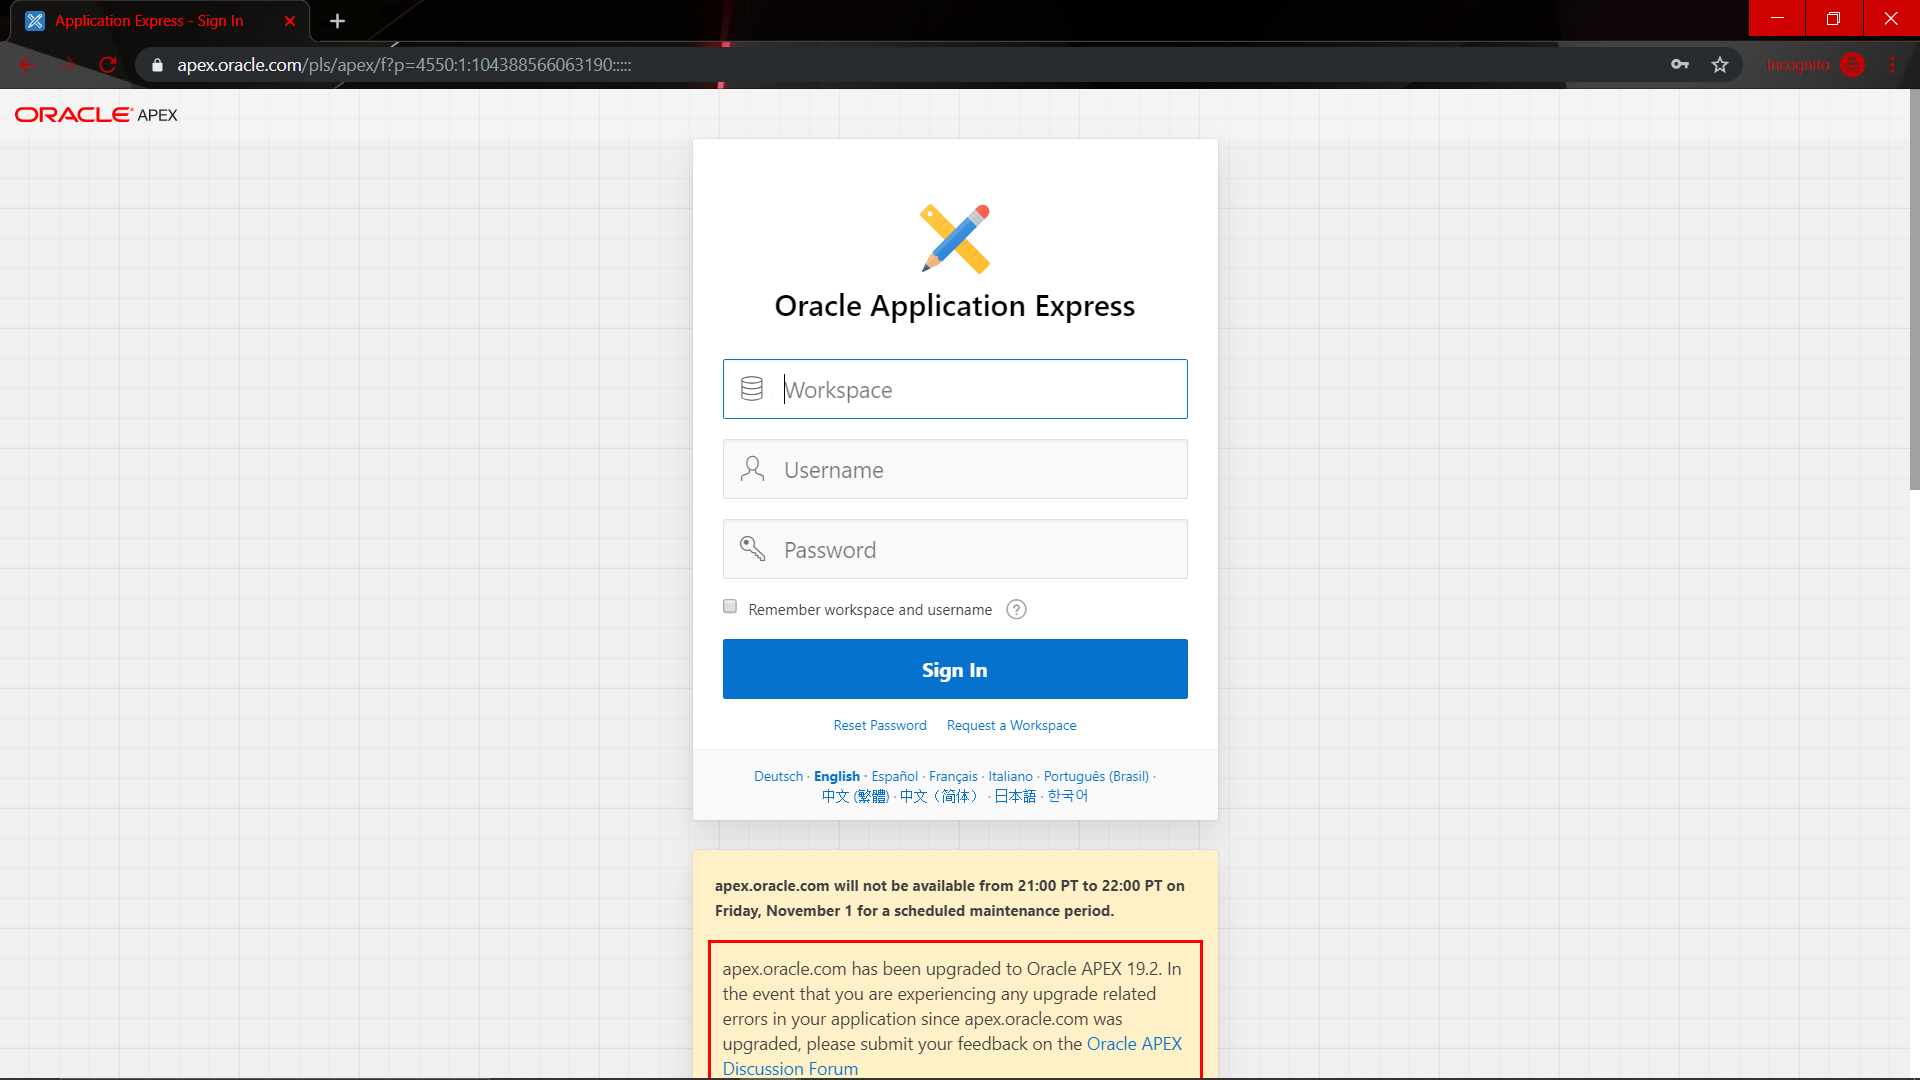
\includegraphics[scale=0.2]{figures/2}}
        \caption{klik reques}
		\label{langkah2}
\end{figure} \\


\item isi request workspace
\begin{figure}[H]
        \centerline{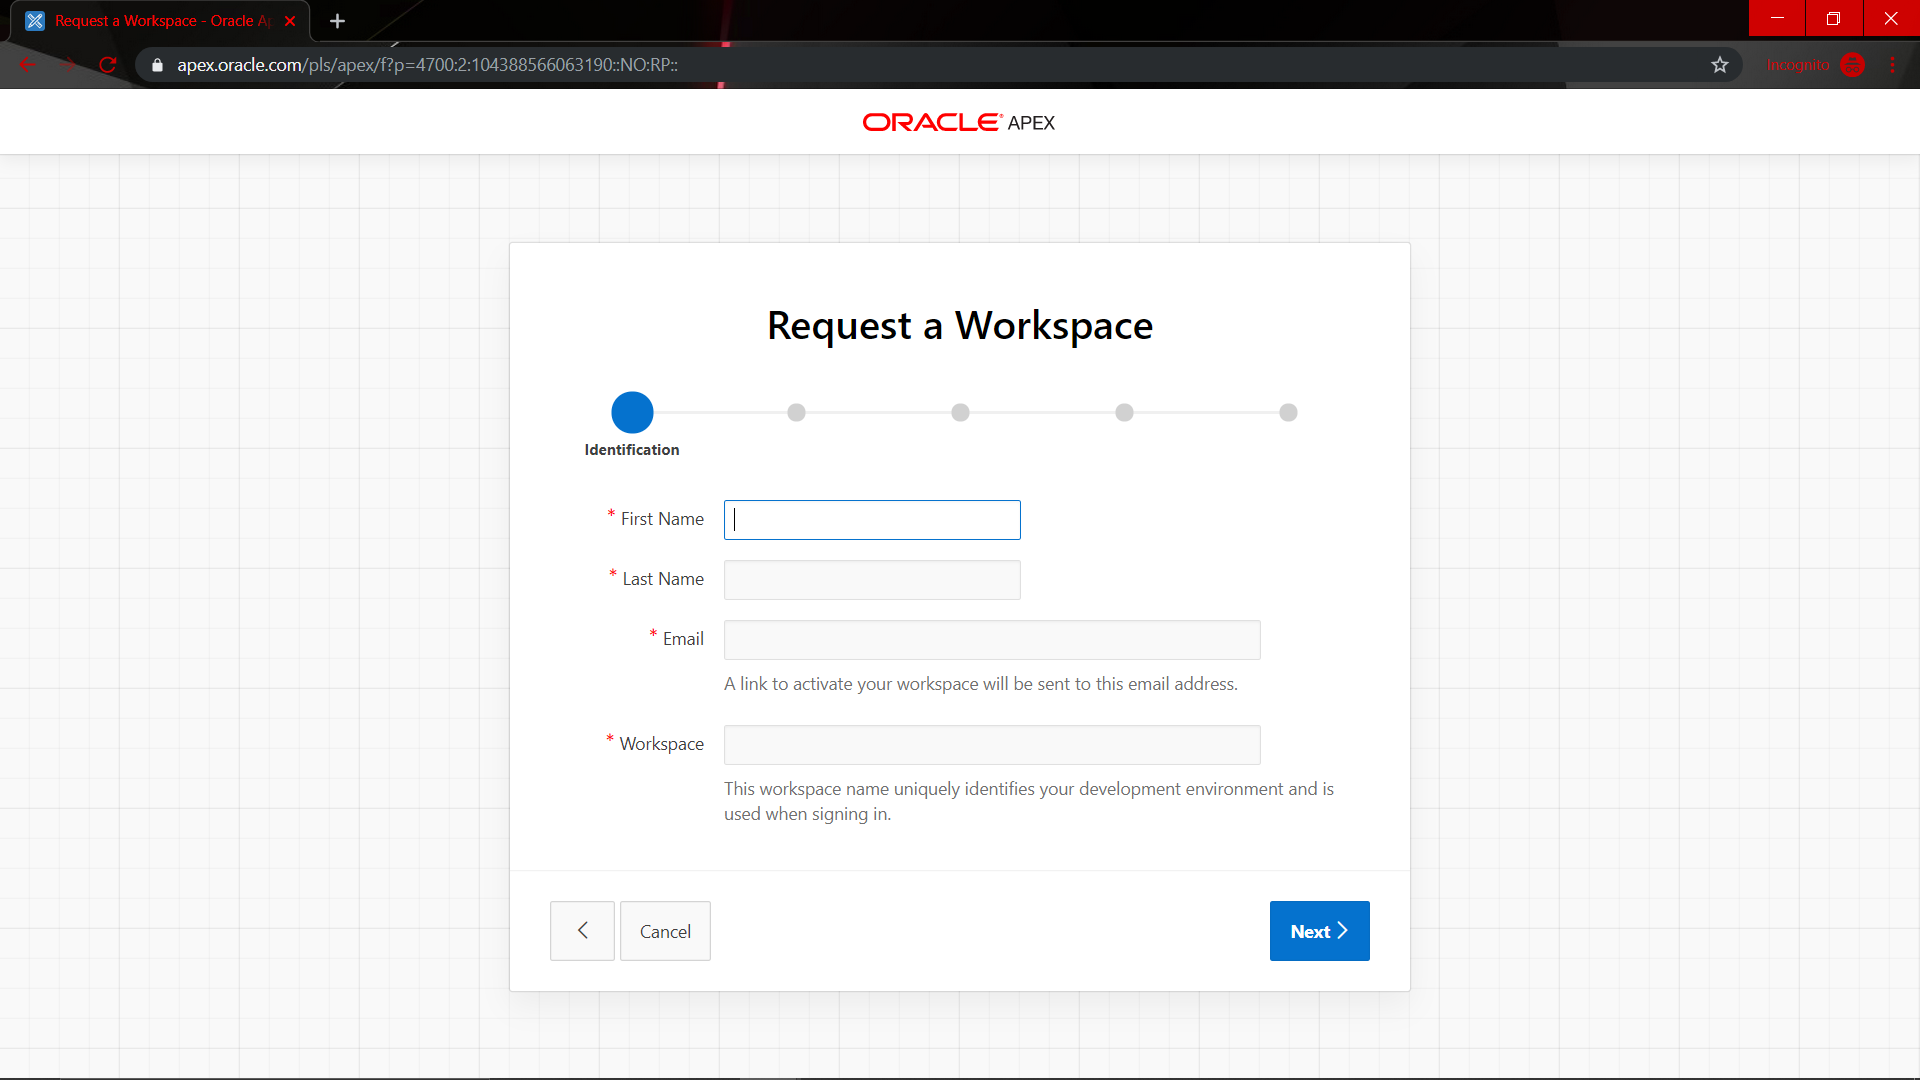
\includegraphics[scale=0.2]{figures/3}}
        \caption{reques workspace}
		\label{langkah2}
\end{figure} \\


\item isi survey

\begin{figure}[H]
    \centering
    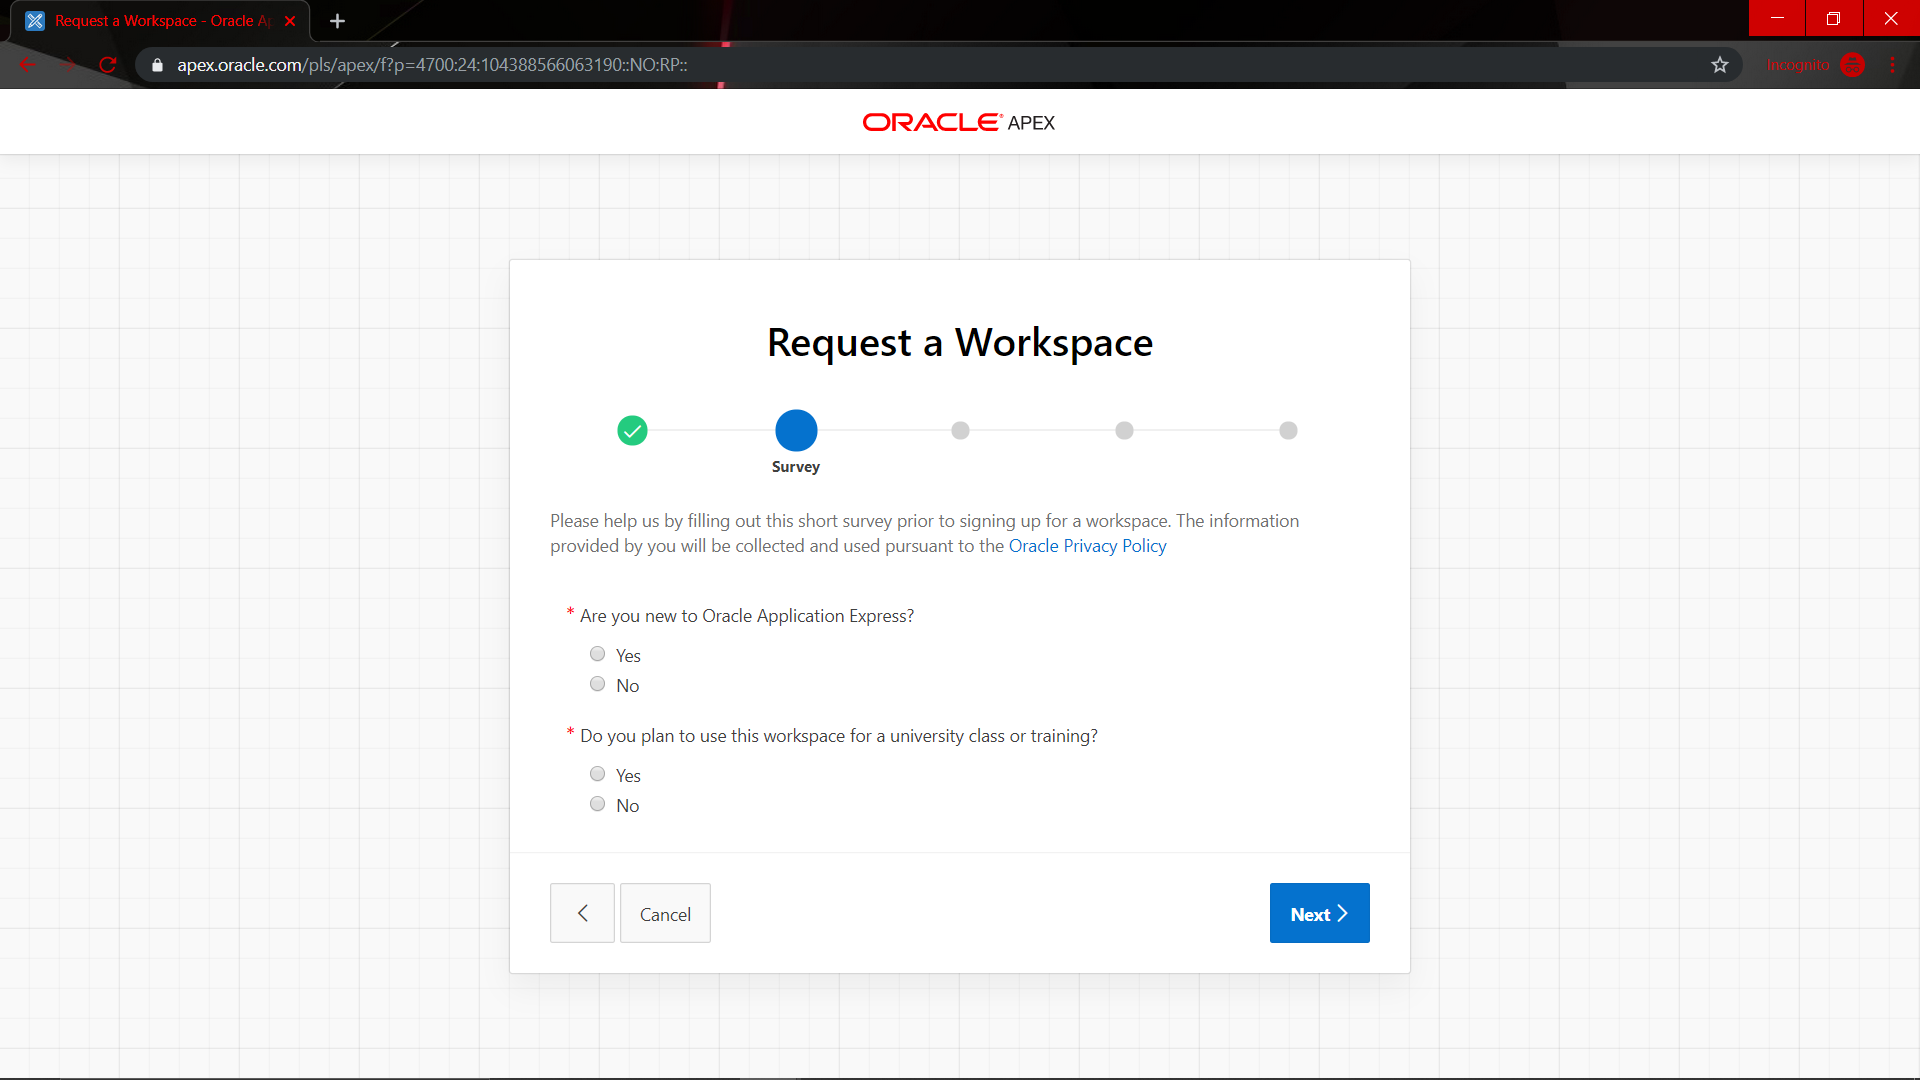
\includegraphics[scale=0.2]{figures/4}
    \caption{isi survey}
    \label{Figureanaconda3}
\end{figure} \\


\item isi justification

\begin{figure}[H]
    \centering
    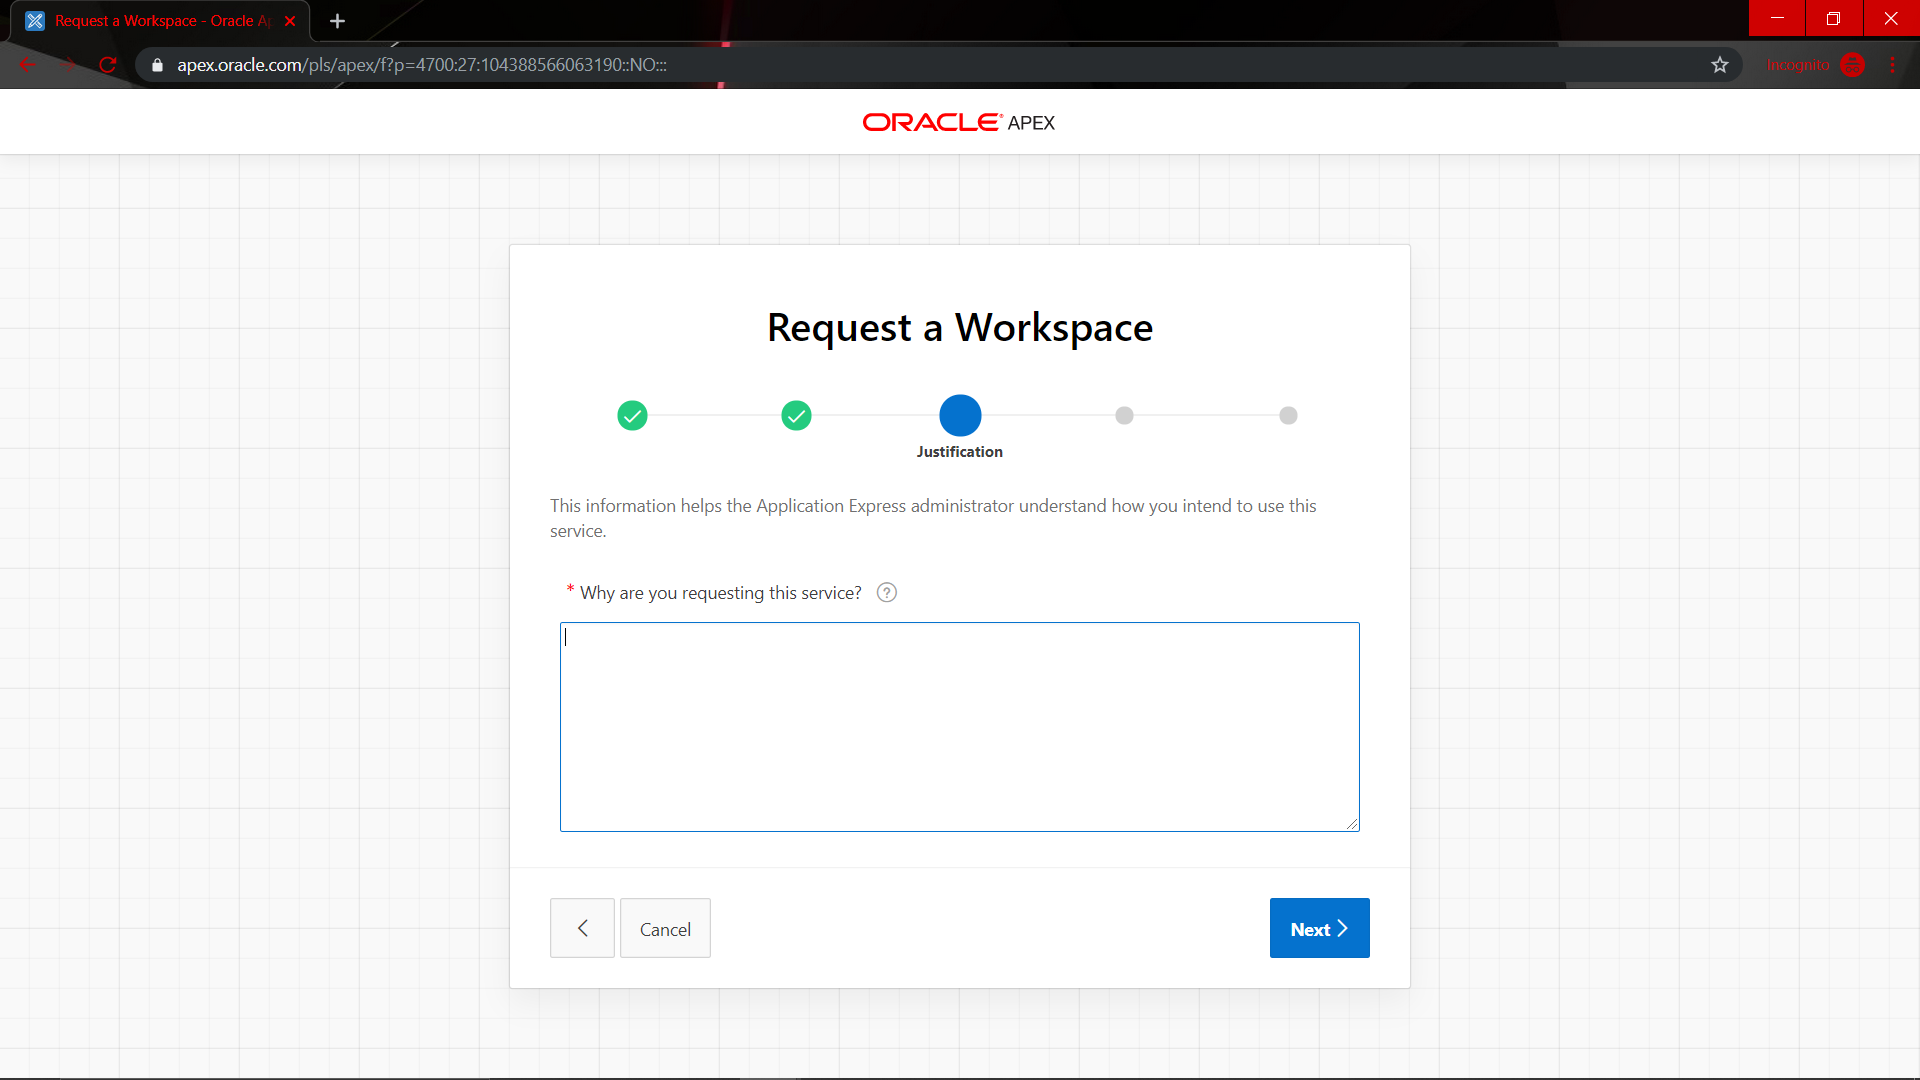
\includegraphics[scale=0.2]{figures/5}
    \caption{isi }
    \label{Figureanaconda4}
\end{figure} \\


\item isi agreement

\begin{figure}[H]
    \centering
    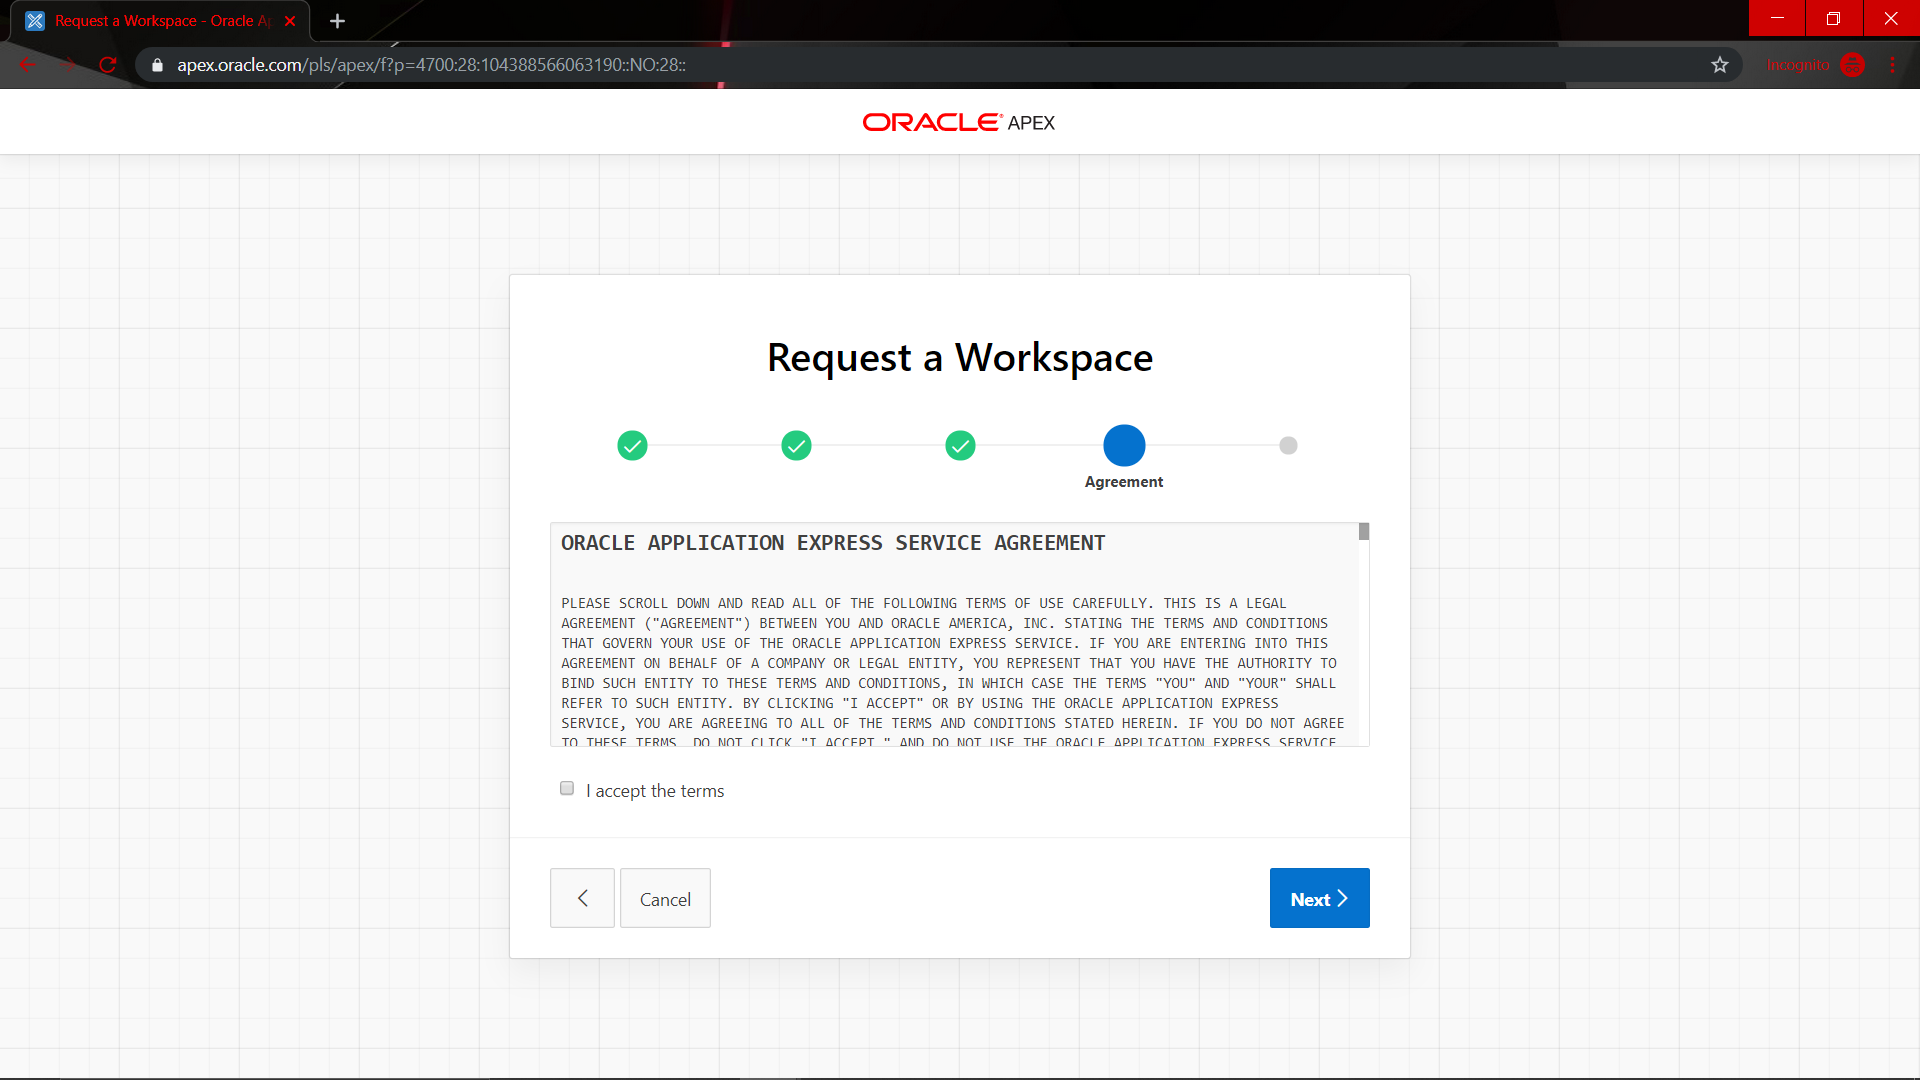
\includegraphics[scale=0.2]{figures/6}
    \caption{klik agreement}
    \label{Figureanaconda5}
\end{figure} \\


\item buka email dan buka email dari oracle karena workspace di approved oleh oracle lalu klik create workspace
\begin{figure}[H]
    \centering
    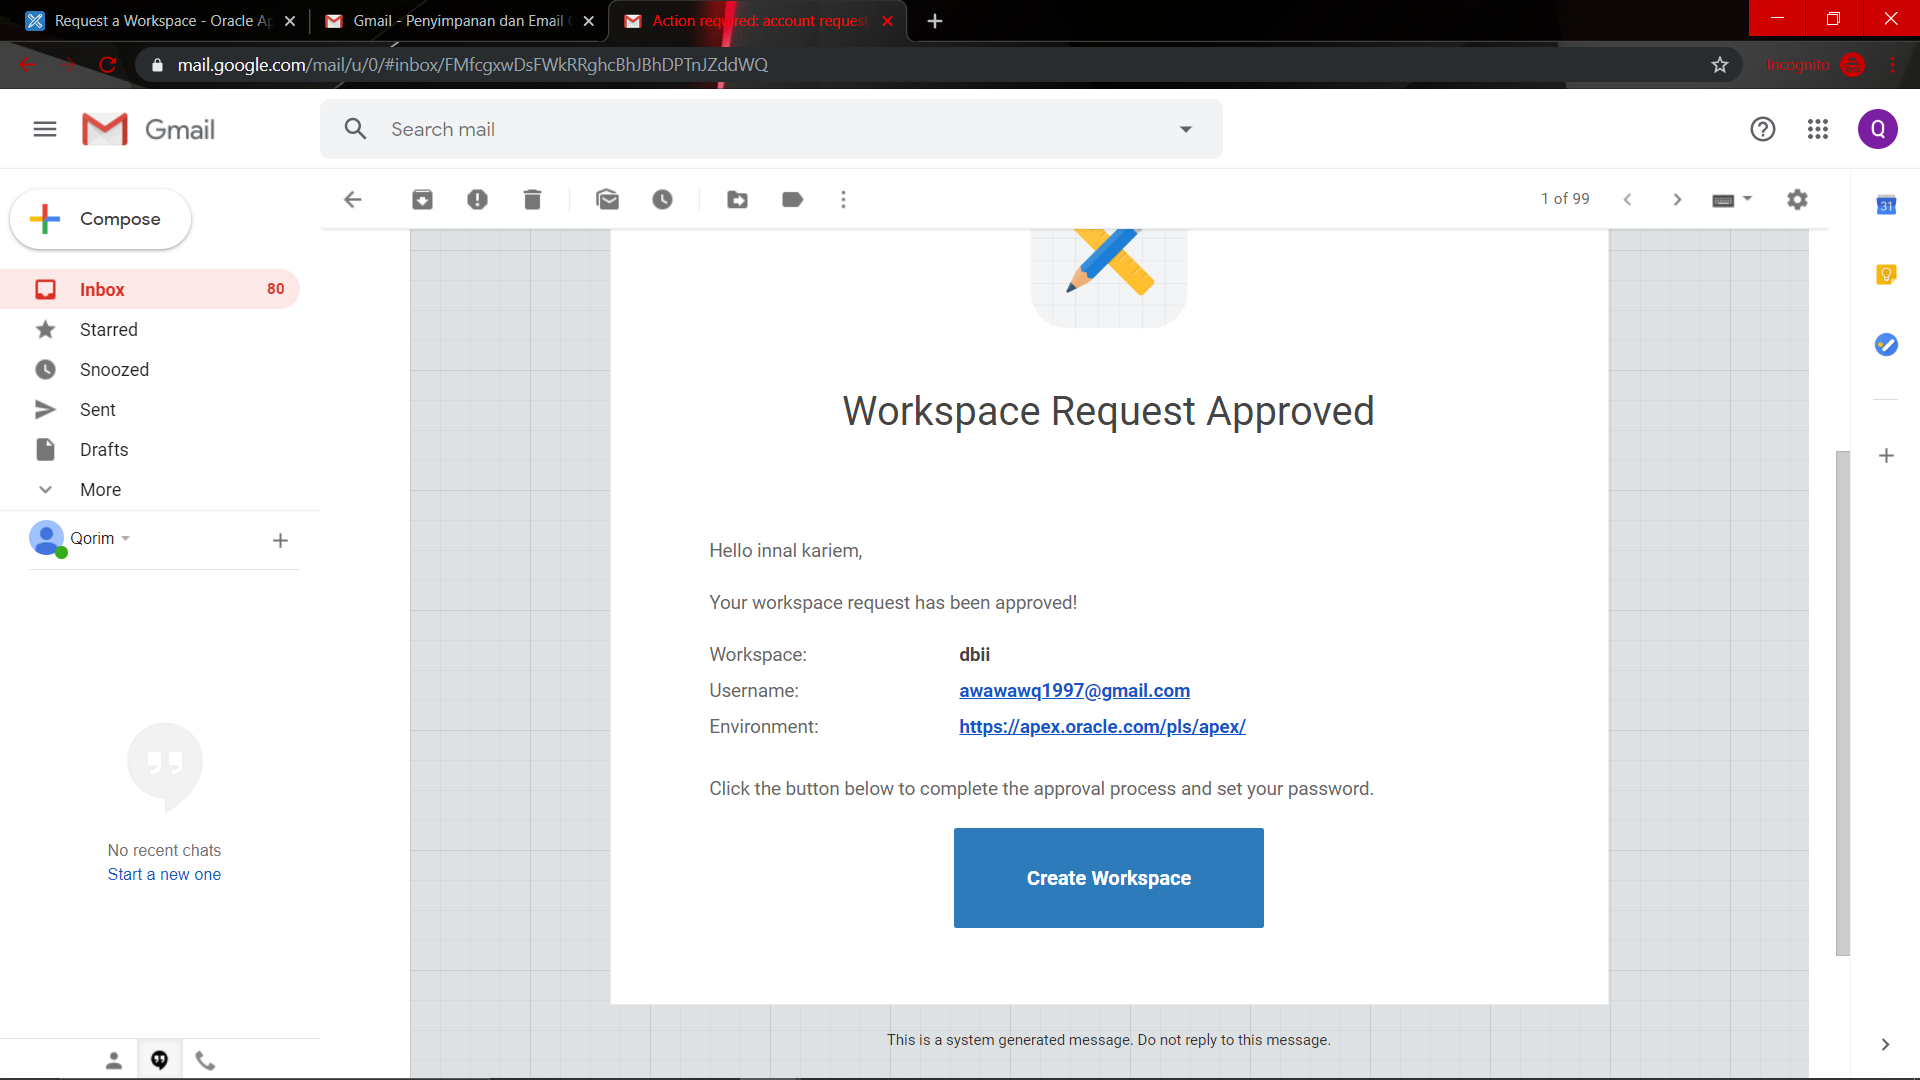
\includegraphics[scale=0.2]{figures/7}
    \caption{Buka email}
    \label{Figureanaconda6}
\end{figure} \\

\item setelah itu akan masuk ke apexnya, lalu masukan password untuk workspace tersebut

\begin{figure}[H]
    \centering
    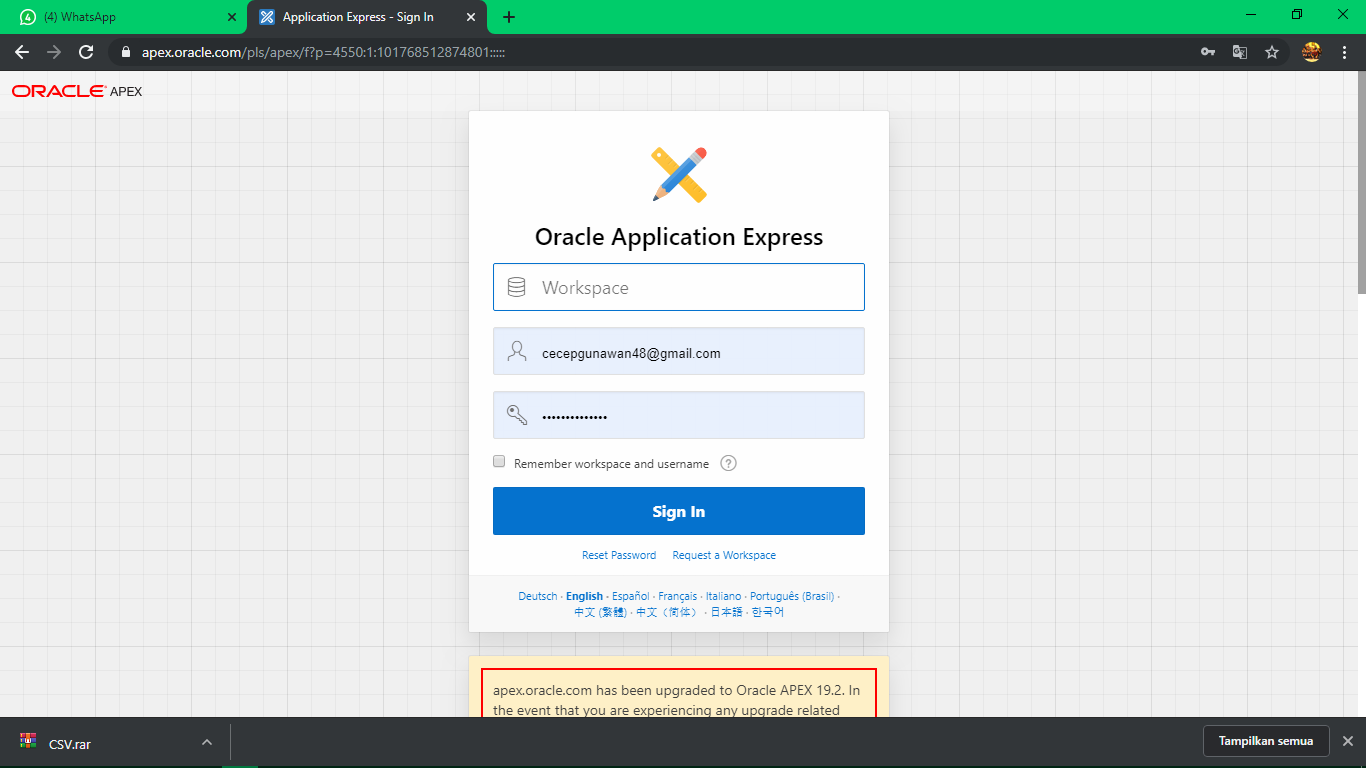
\includegraphics[scale=0.4]{figures/111}
    \caption{Masukan password}
    \label{Figureanaconda7}
\end{figure} \\

\item klik app builder
\begin{figure}[H]
    \centering
    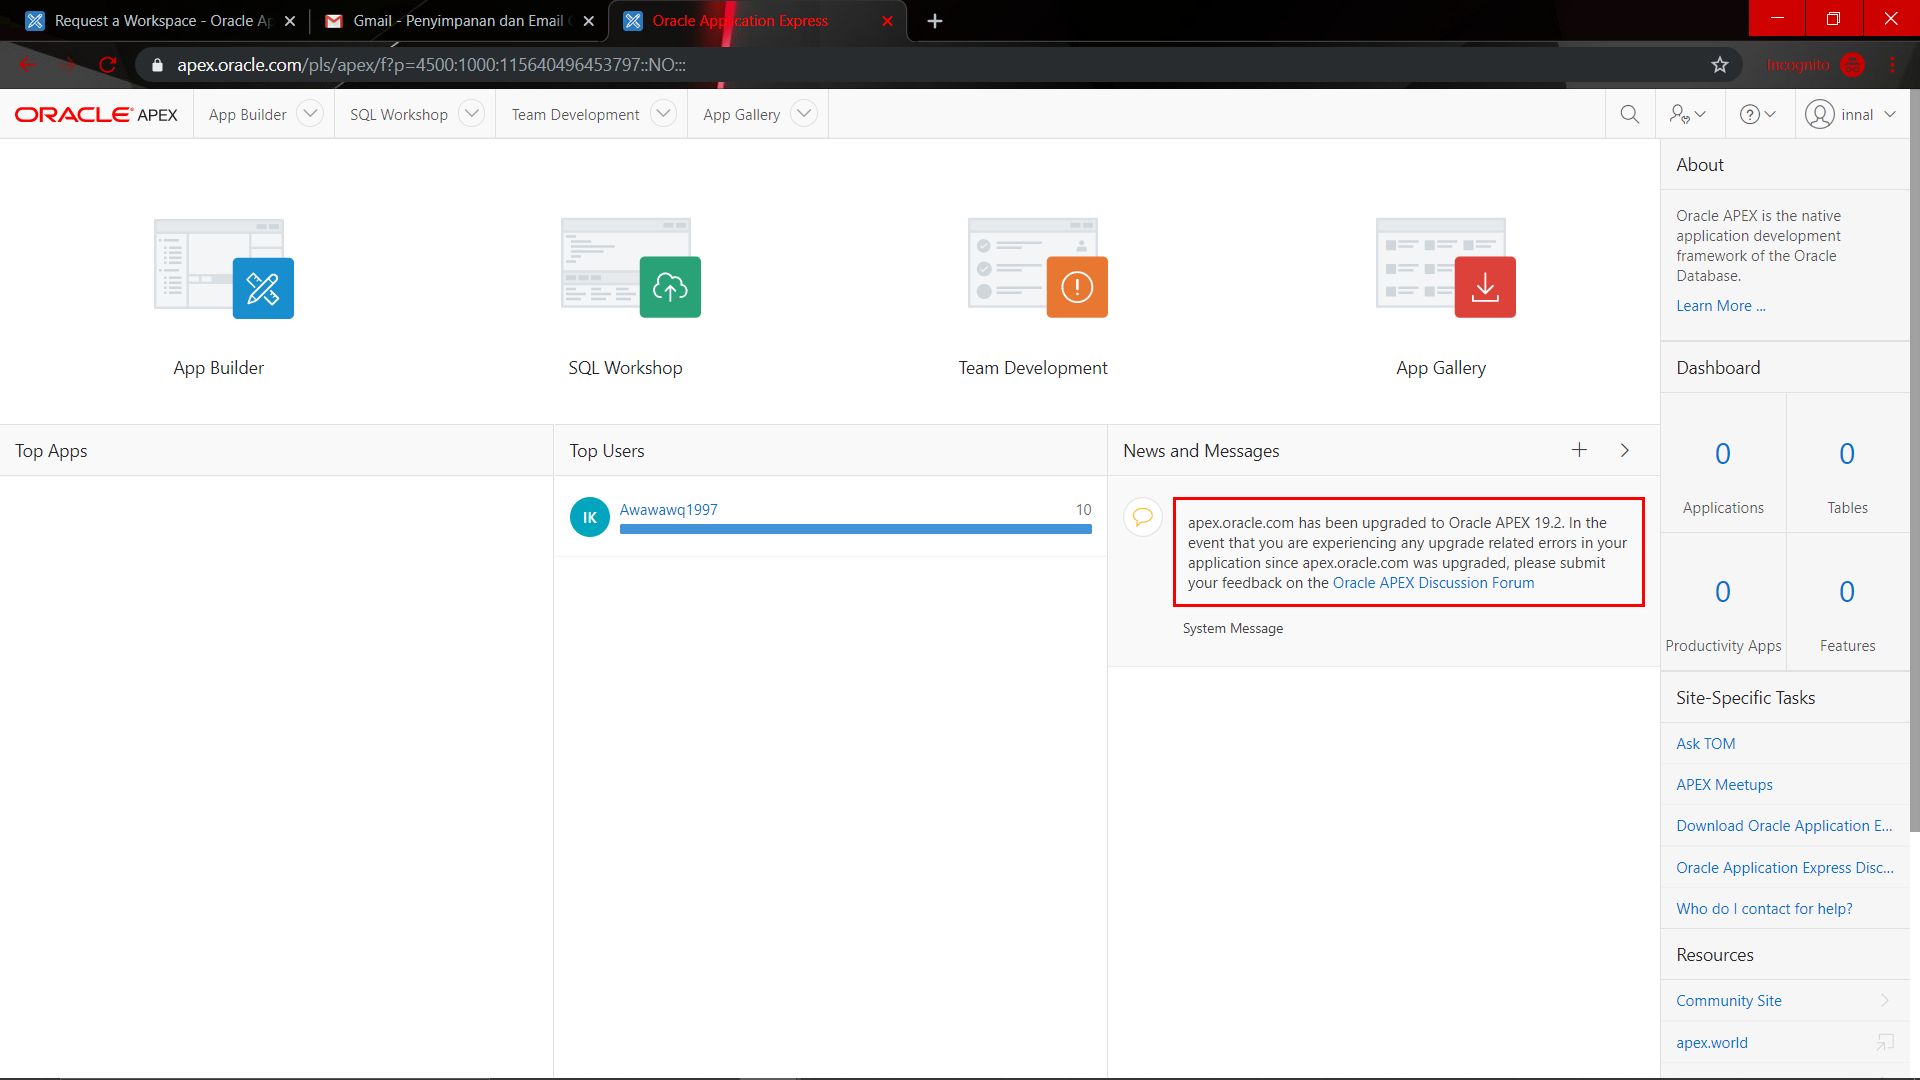
\includegraphics[scale=0.2]{figures/9}
    \caption{App builder}
    \label{Figureanaconda8}
\end{figure} \\

\item klik create 
\begin{figure}[H]
    \centering
    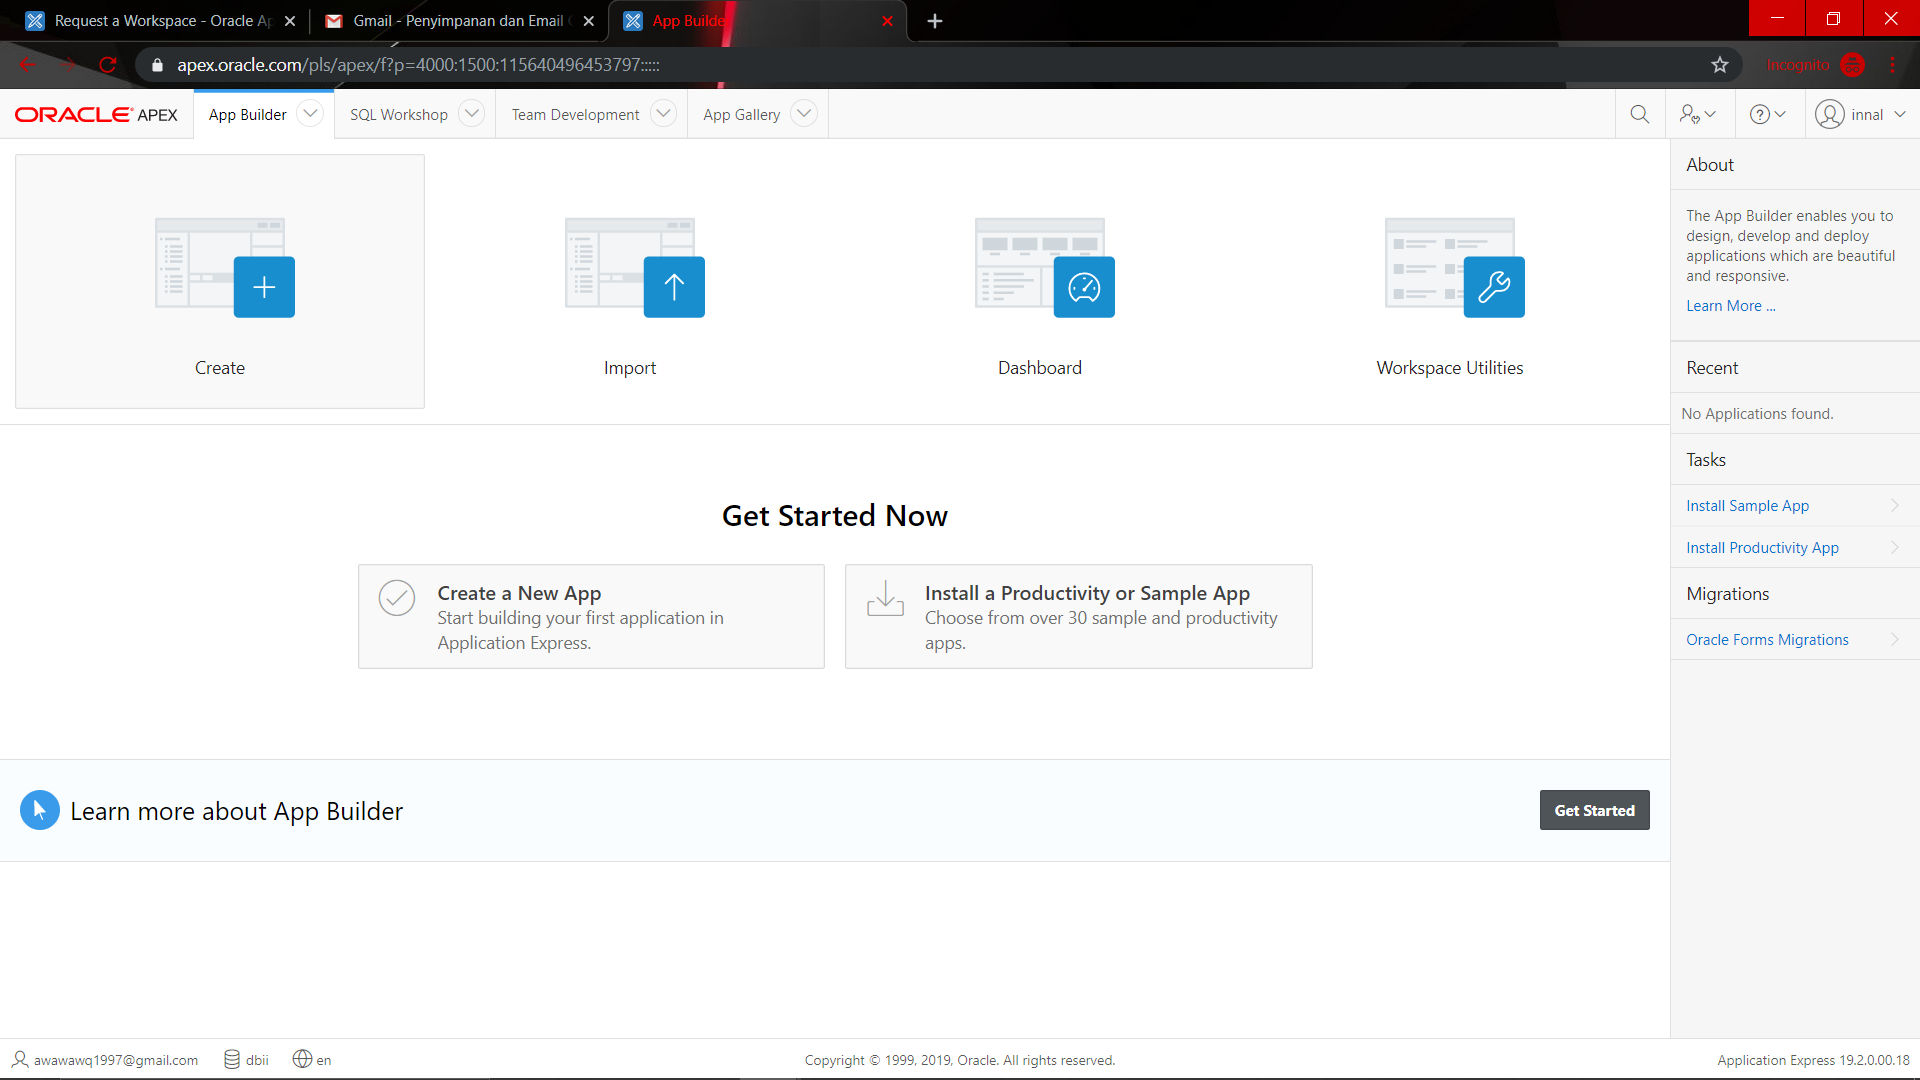
\includegraphics[scale=0.2]{figures/10}
    \caption{Creat }
    \label{Figureanaconda70}
\end{figure} \\

\item klik from a file

\begin{figure}[H]
    \centering
    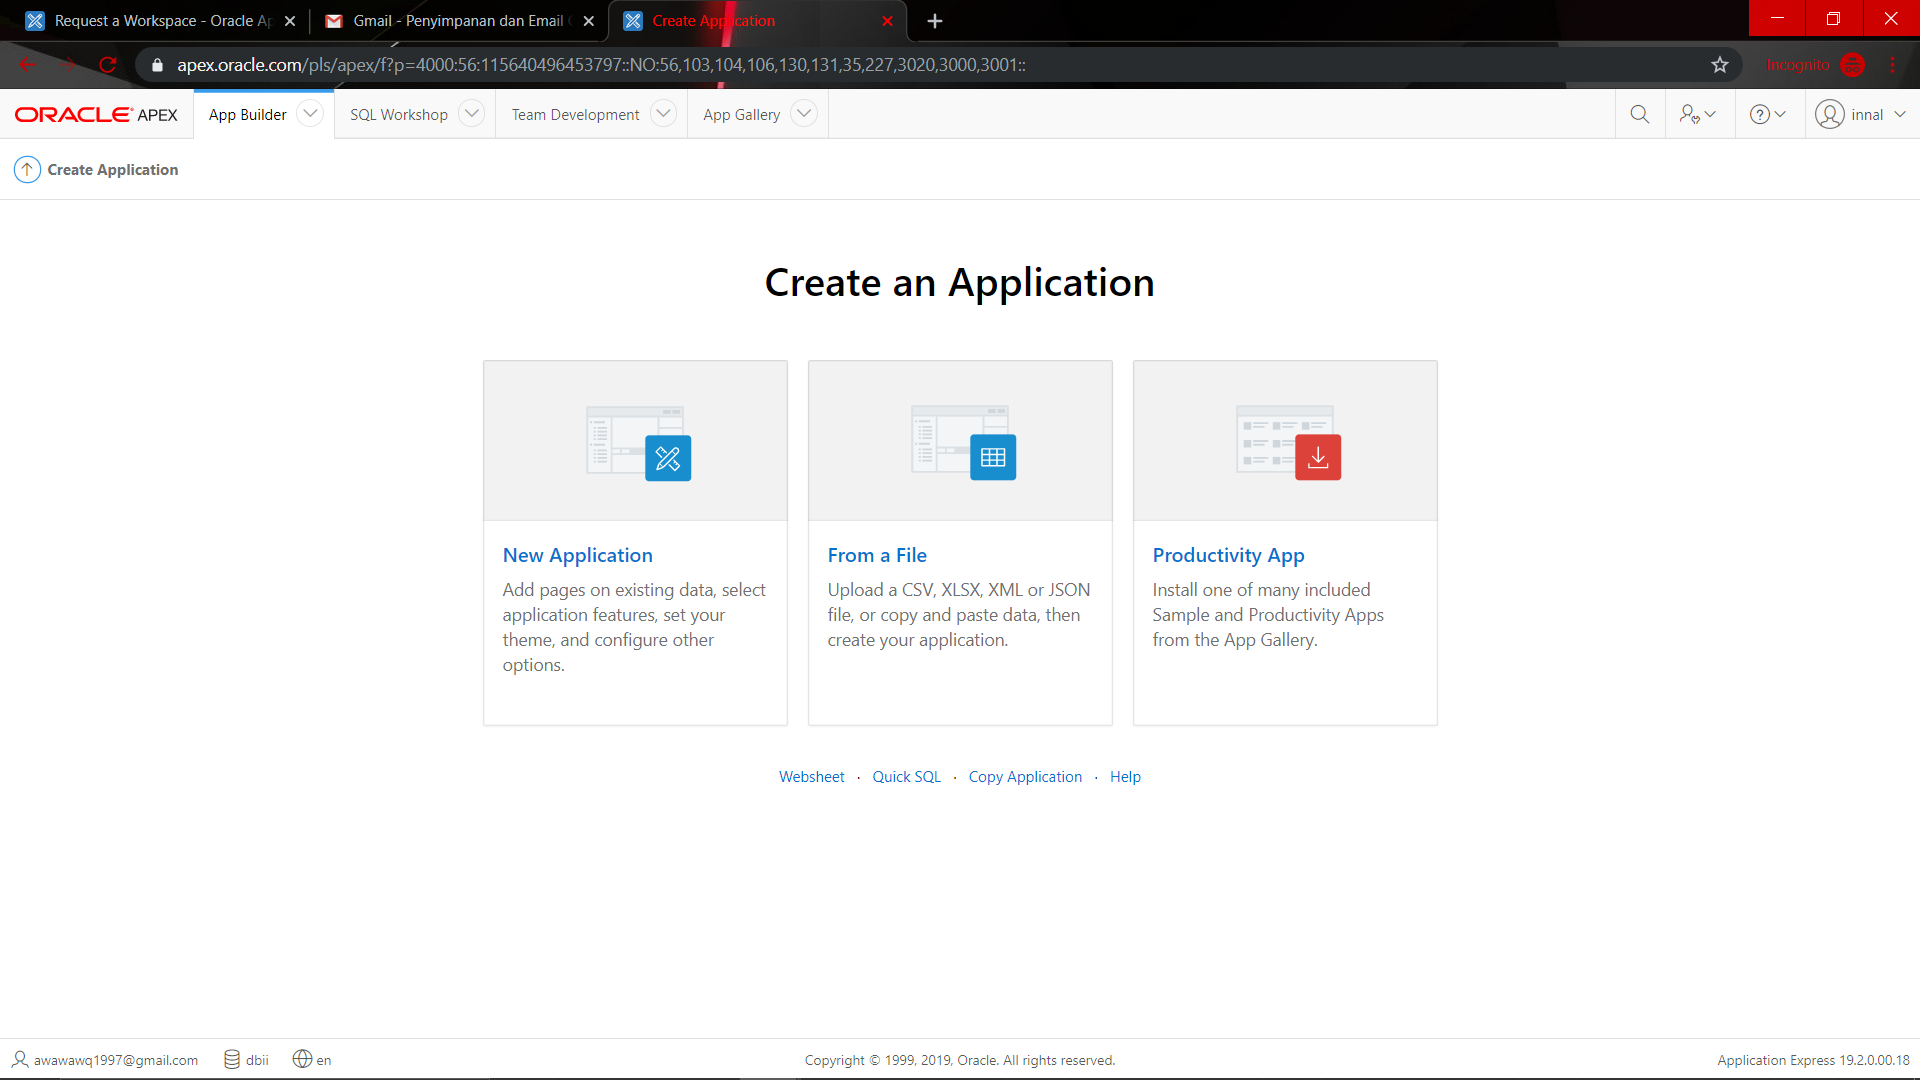
\includegraphics[scale=0.2]{figures/11}
    \caption{From a file}
    \label{Figureanaconda70}
\end{figure}
\item masukan file 

\begin{figure}[H]
    \centering
    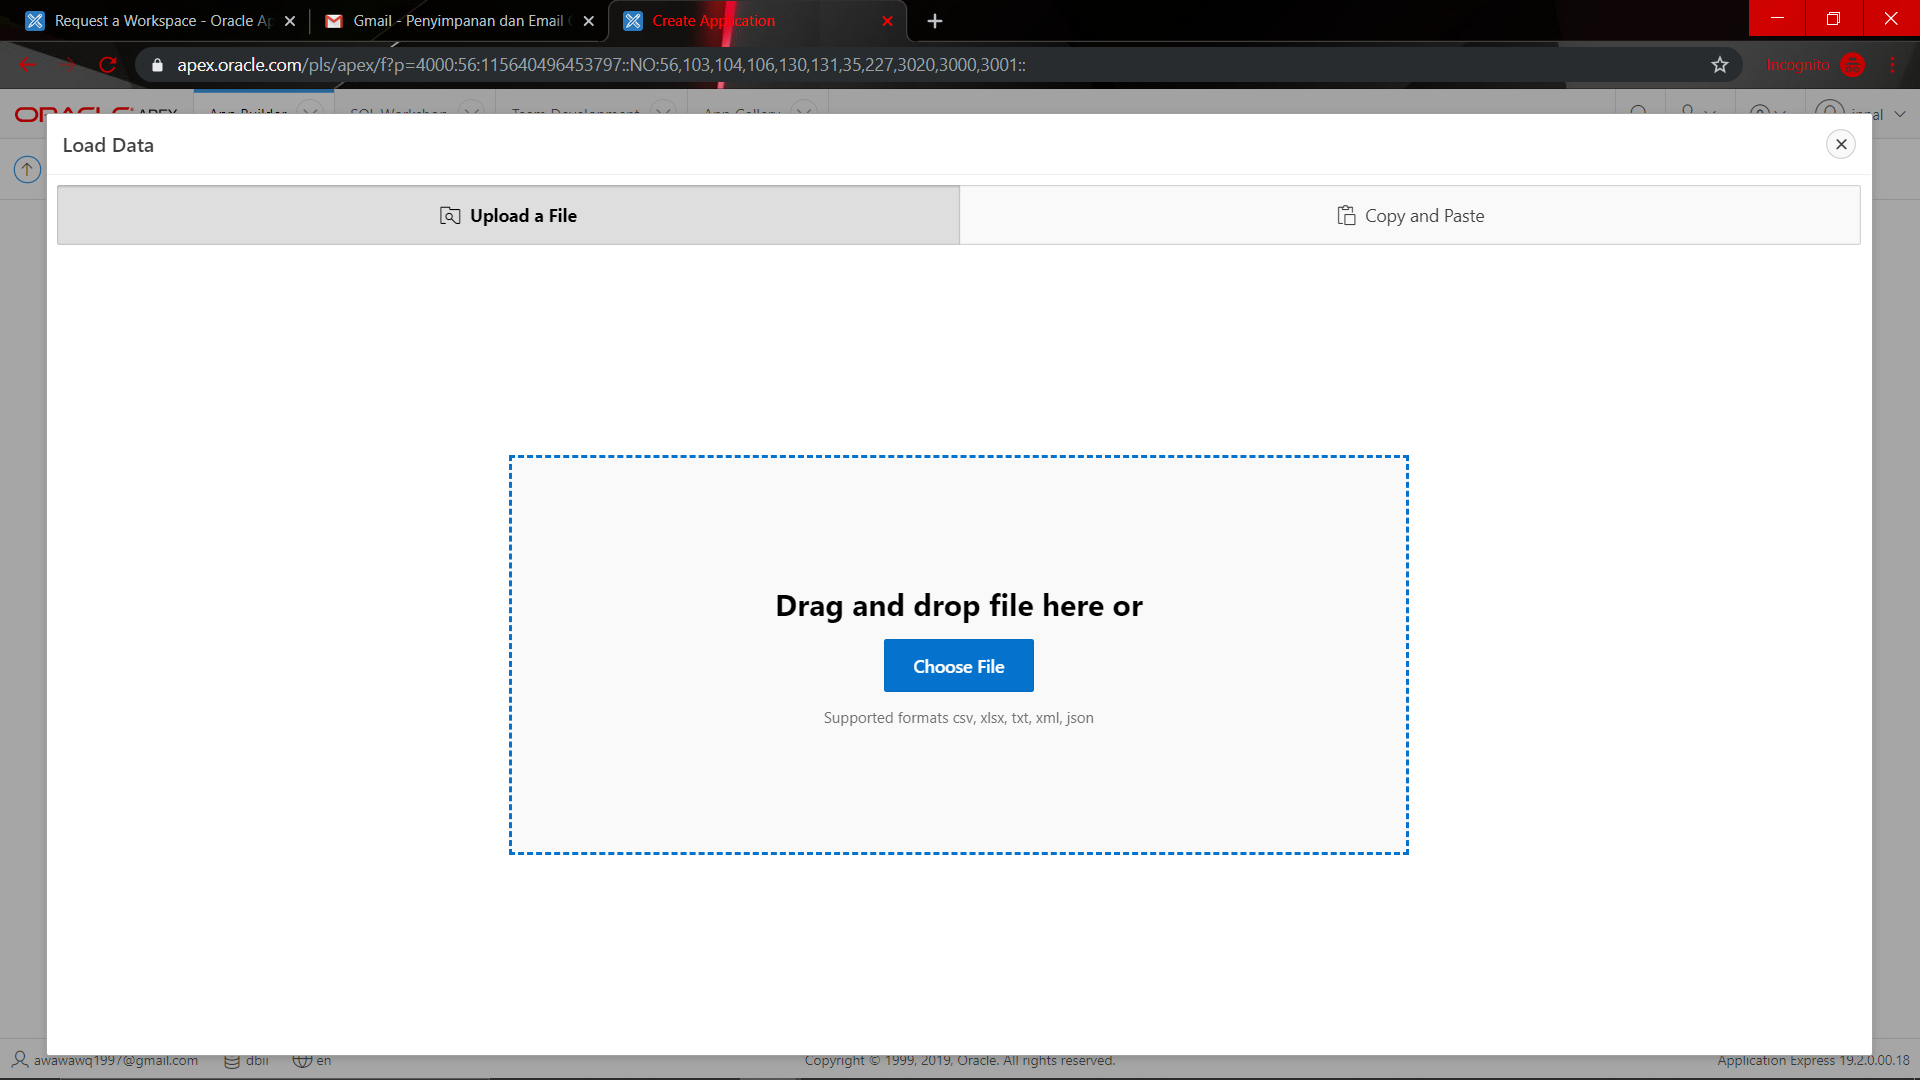
\includegraphics[scale=0.2]{figures/14}
    \caption{Masukan file}
    \label{Figureanaconda70}
\end{figure} \\


\item berikan nama untuk file tersebut dan klik load data
\begin{figure}[H]
    \centering
    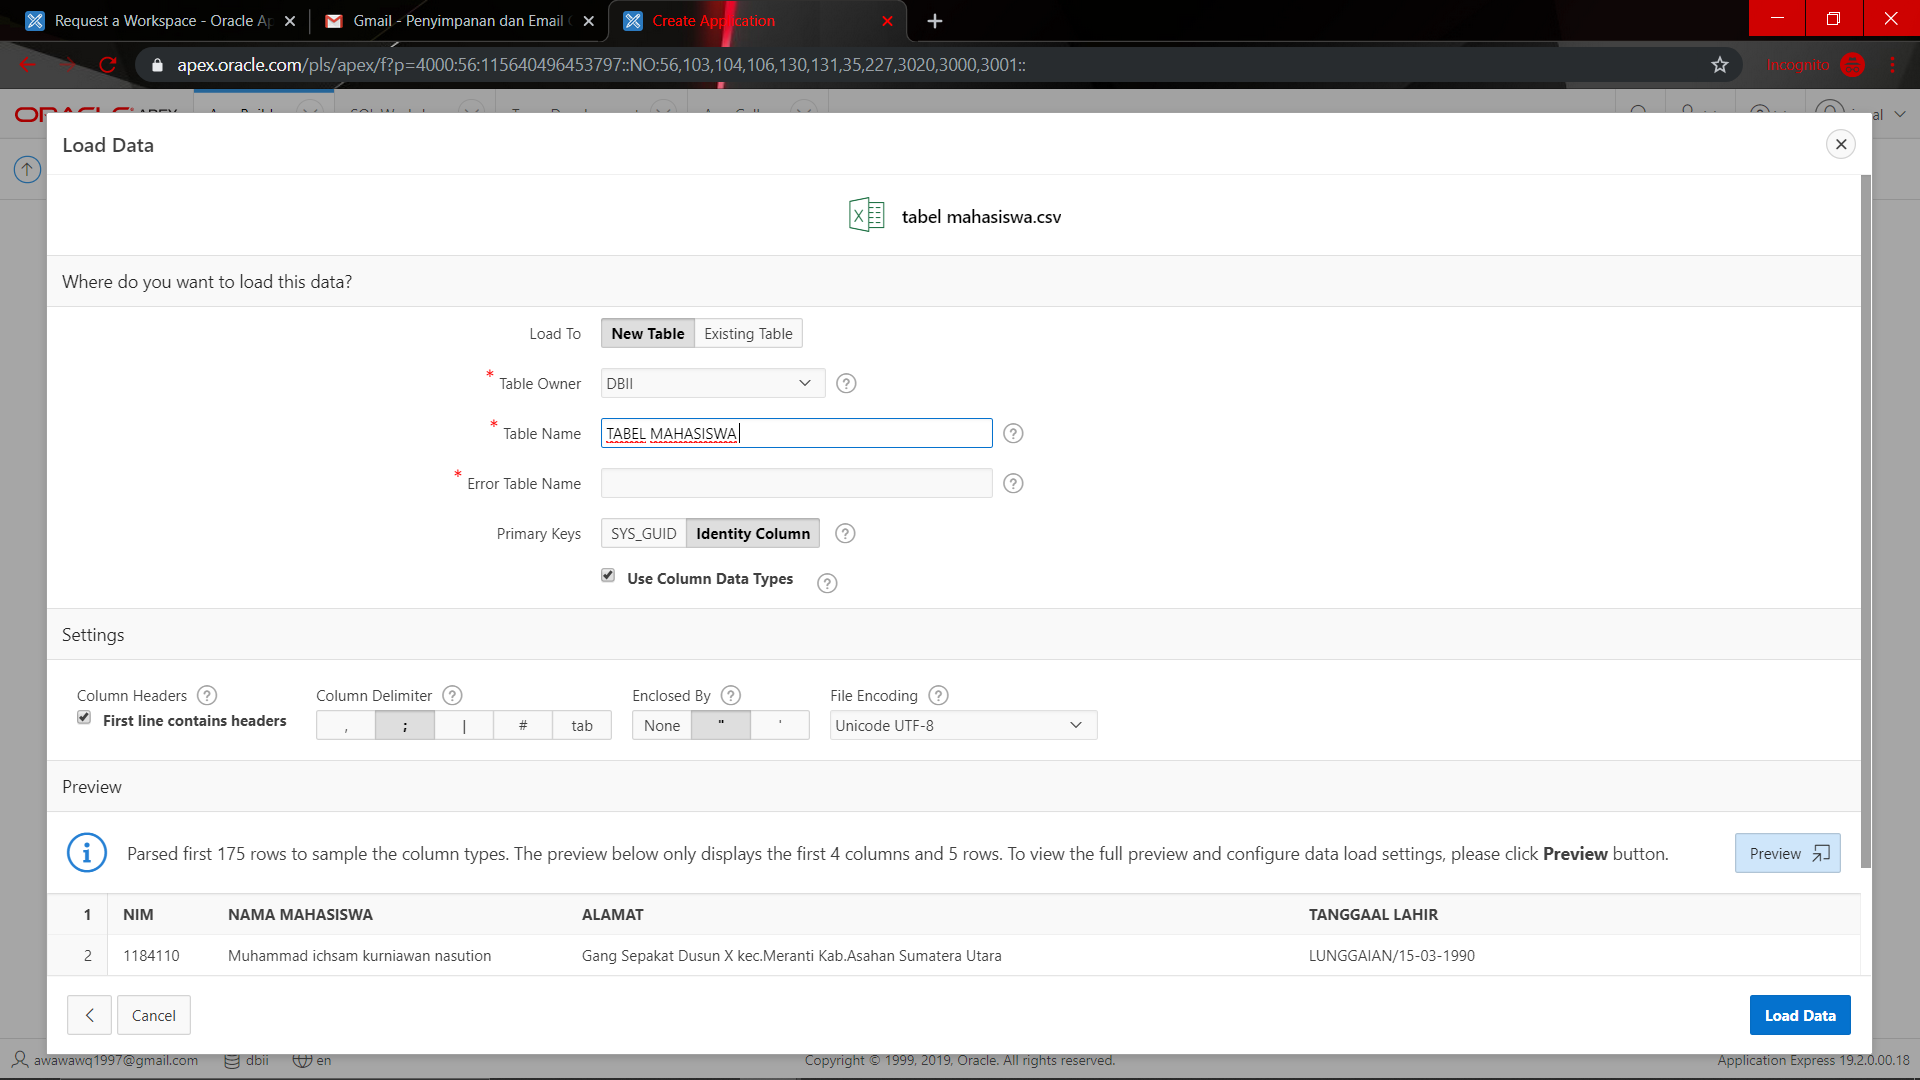
\includegraphics[scale=0.2]{figures/12}
    \caption{Nama untuk file}
    \label{Figureanaconda70}
\end{figure} \\

\item klik from a file 
\begin{figure}[H]
    \centering
    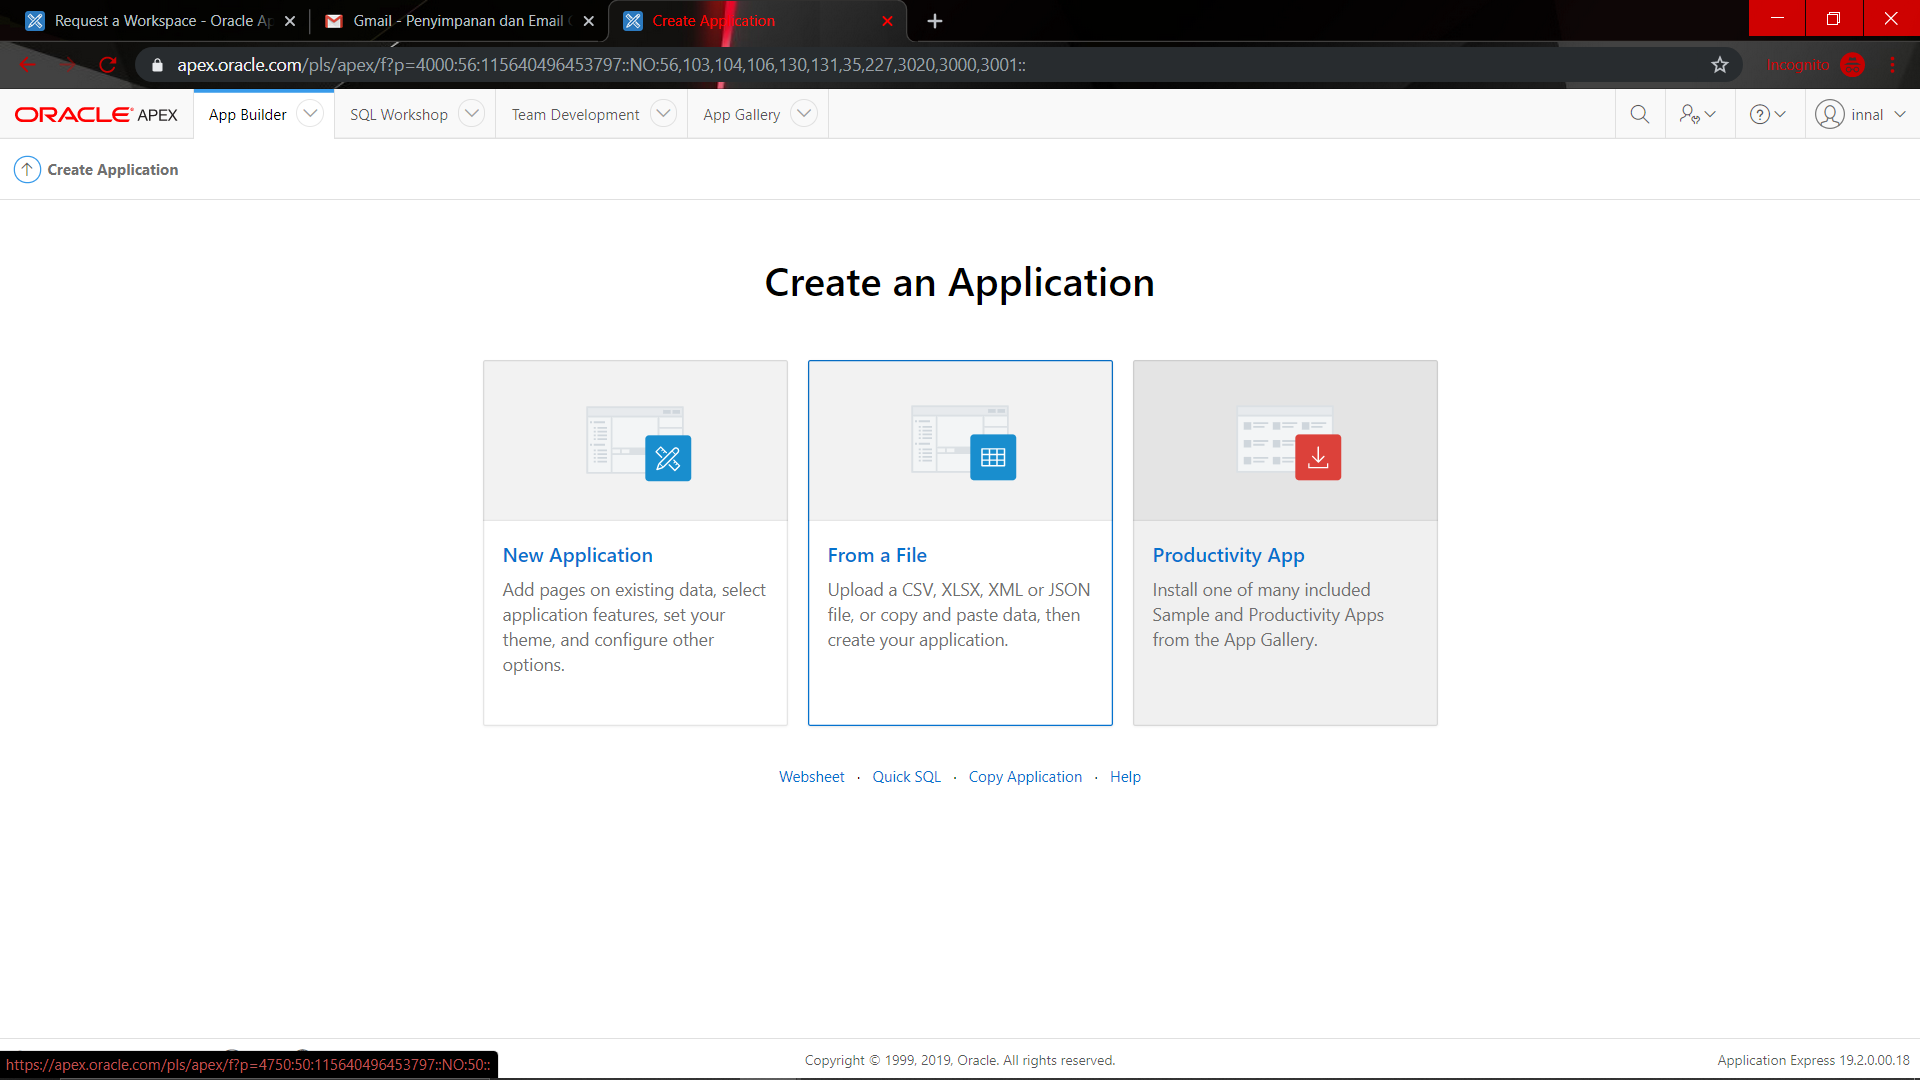
\includegraphics[scale=0.2]{figures/13}
    \caption{Klik from a file}
    \label{Figureanaconda70}
\end{figure} \\

\item masukan file lain yang ingin dimasukan 
\begin{figure}[H]
    \centering
    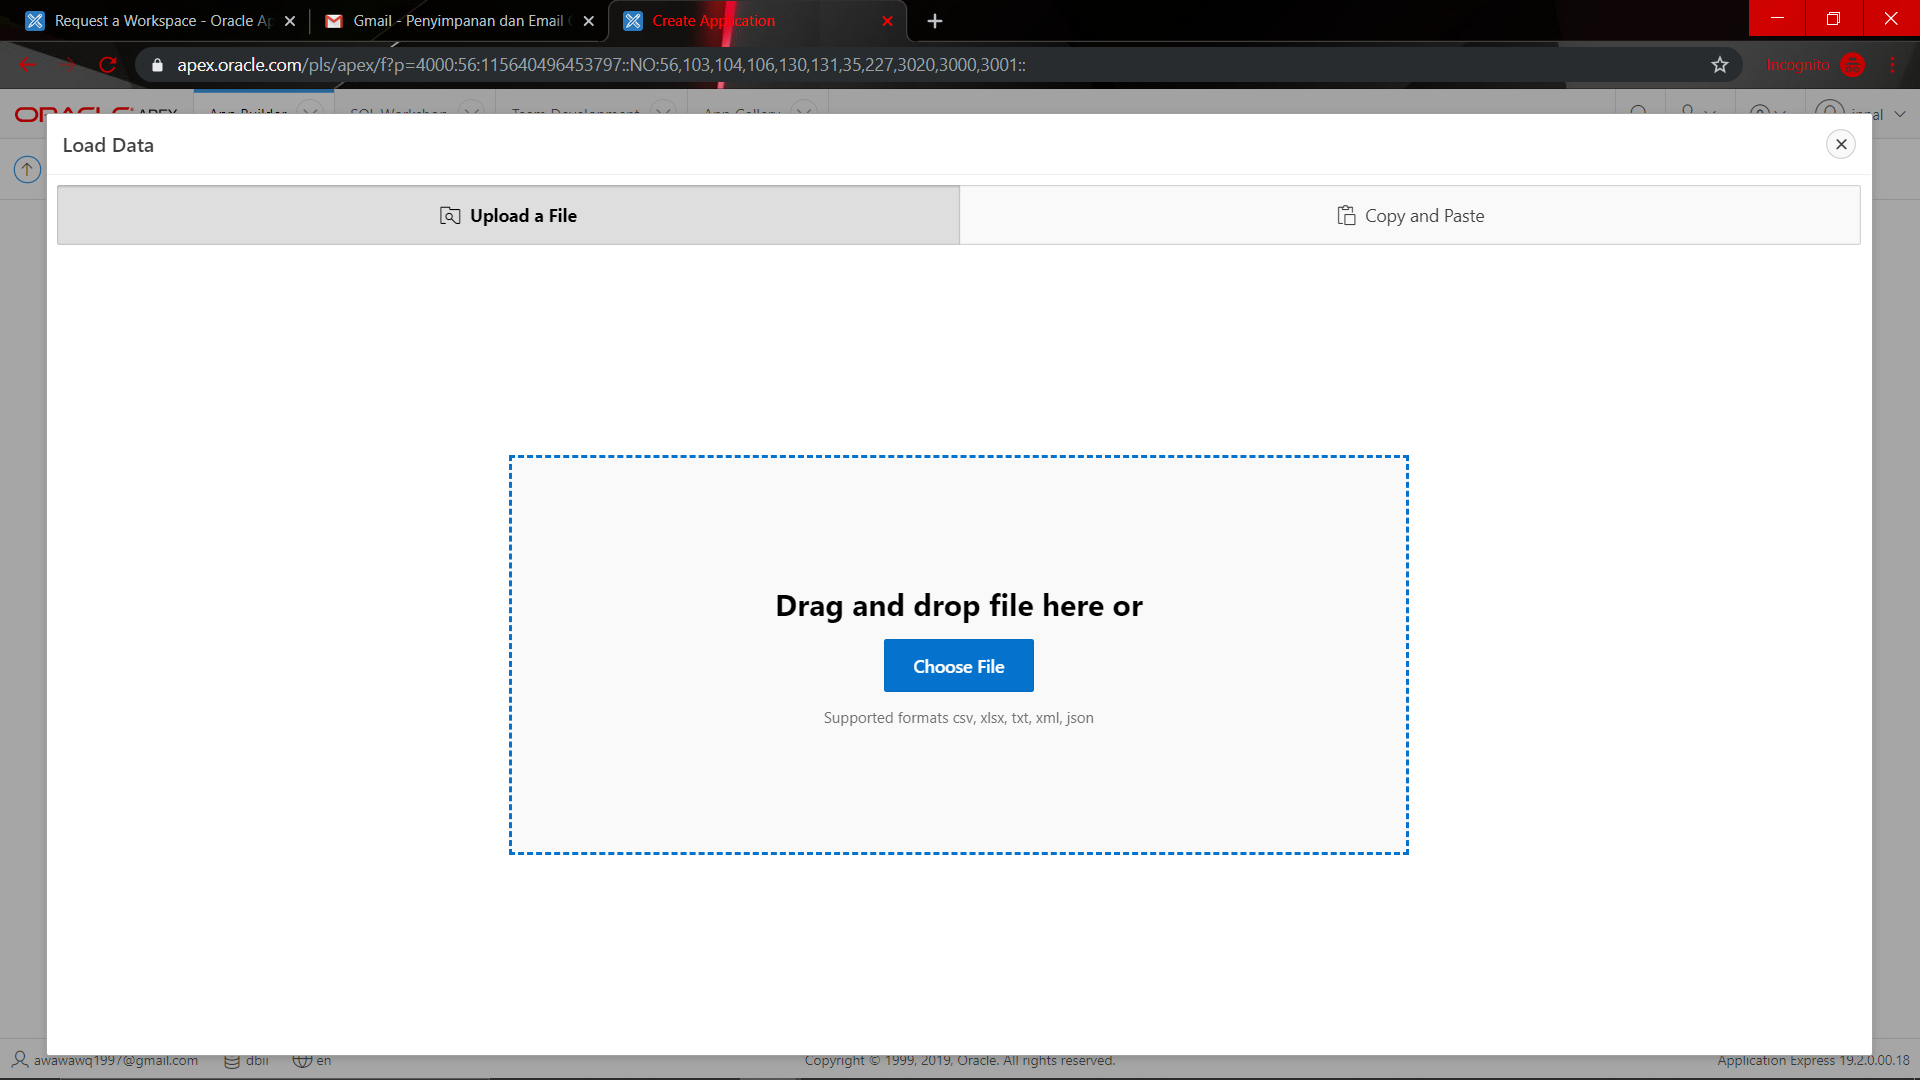
\includegraphics[scale=0.2]{figures/14}
    \caption{Masukan file}
    \label{Figureanaconda70}
\end{figure} \\


\item berikan nama untuk file tersebut 
\begin{figure}[H]
    \centering
    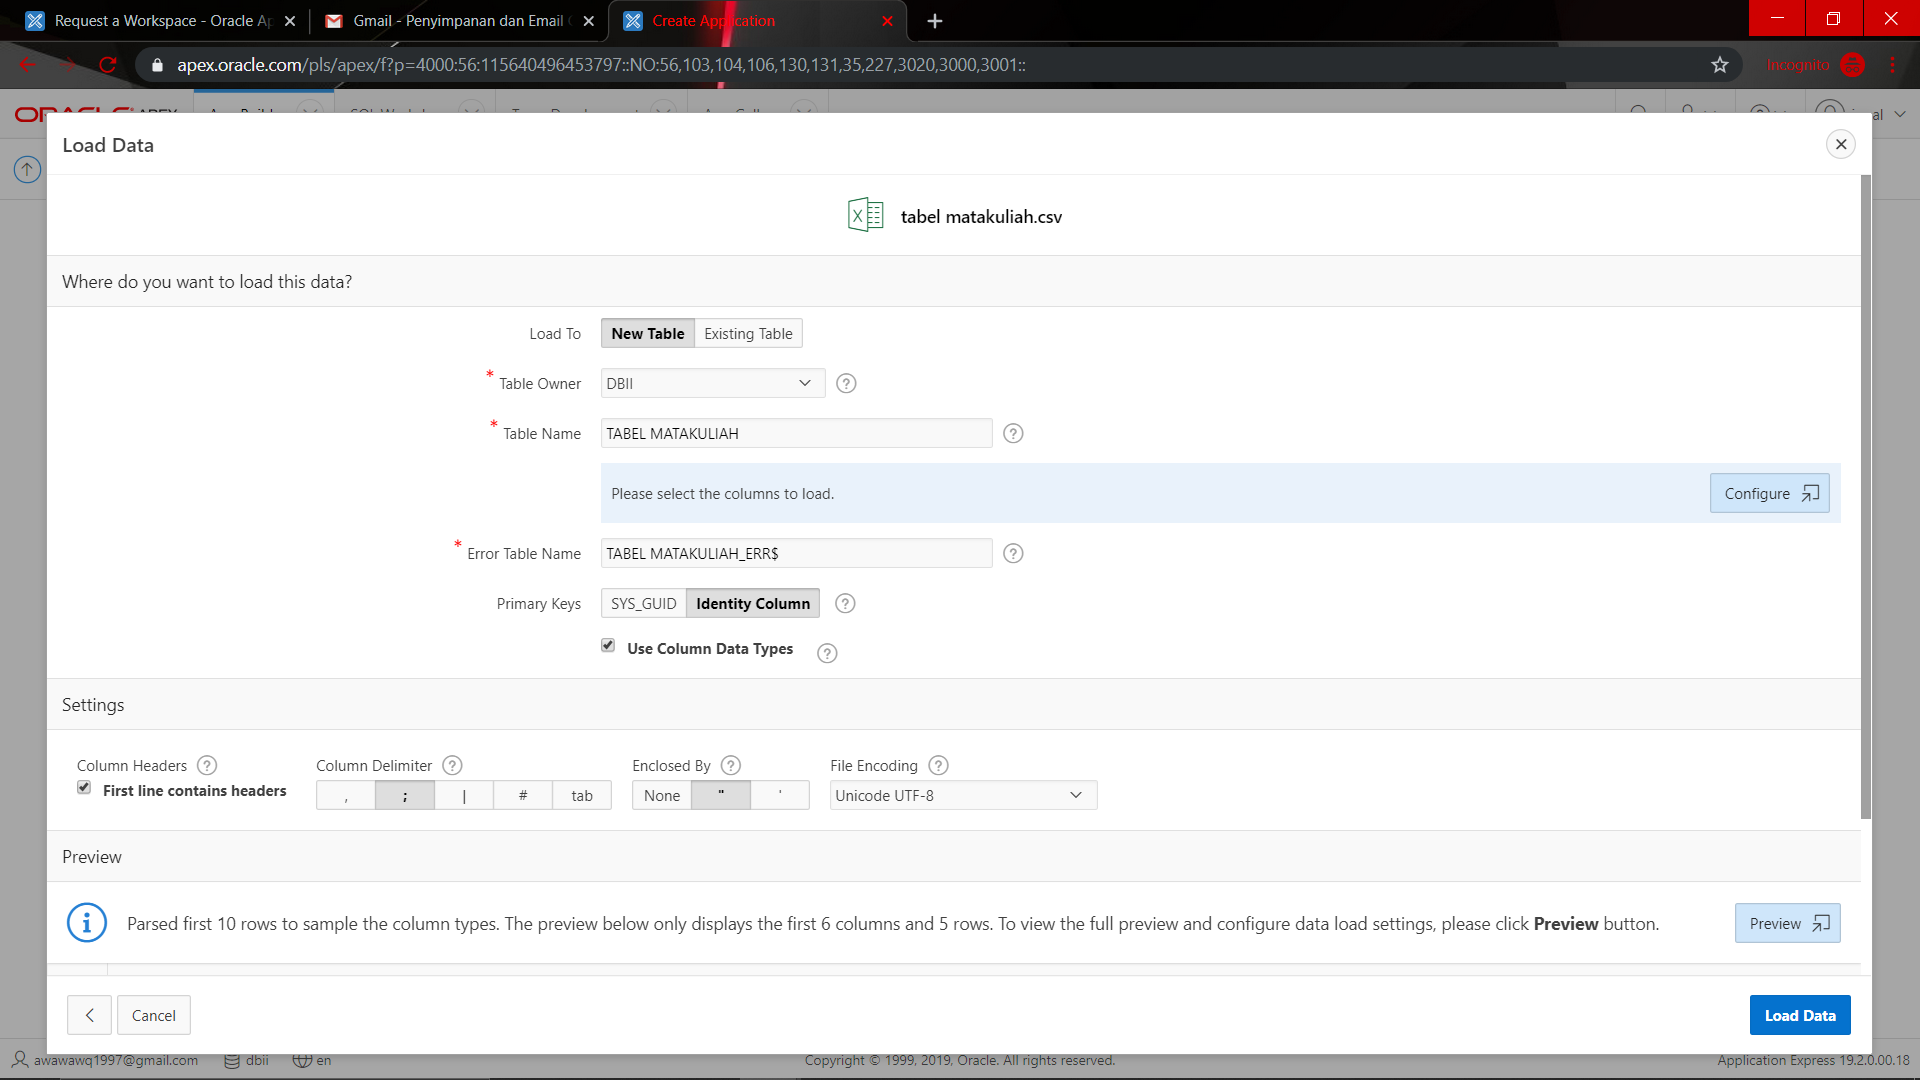
\includegraphics[scale=0.2]{figures/15}
    \caption{Berikan nama file}
    \label{Environment1}
\end{figure} \\
 
\item untuk melihat file tabel yang sudah dimasukan klik error table dan klik configure
\begin{figure}[H]
    \centering
    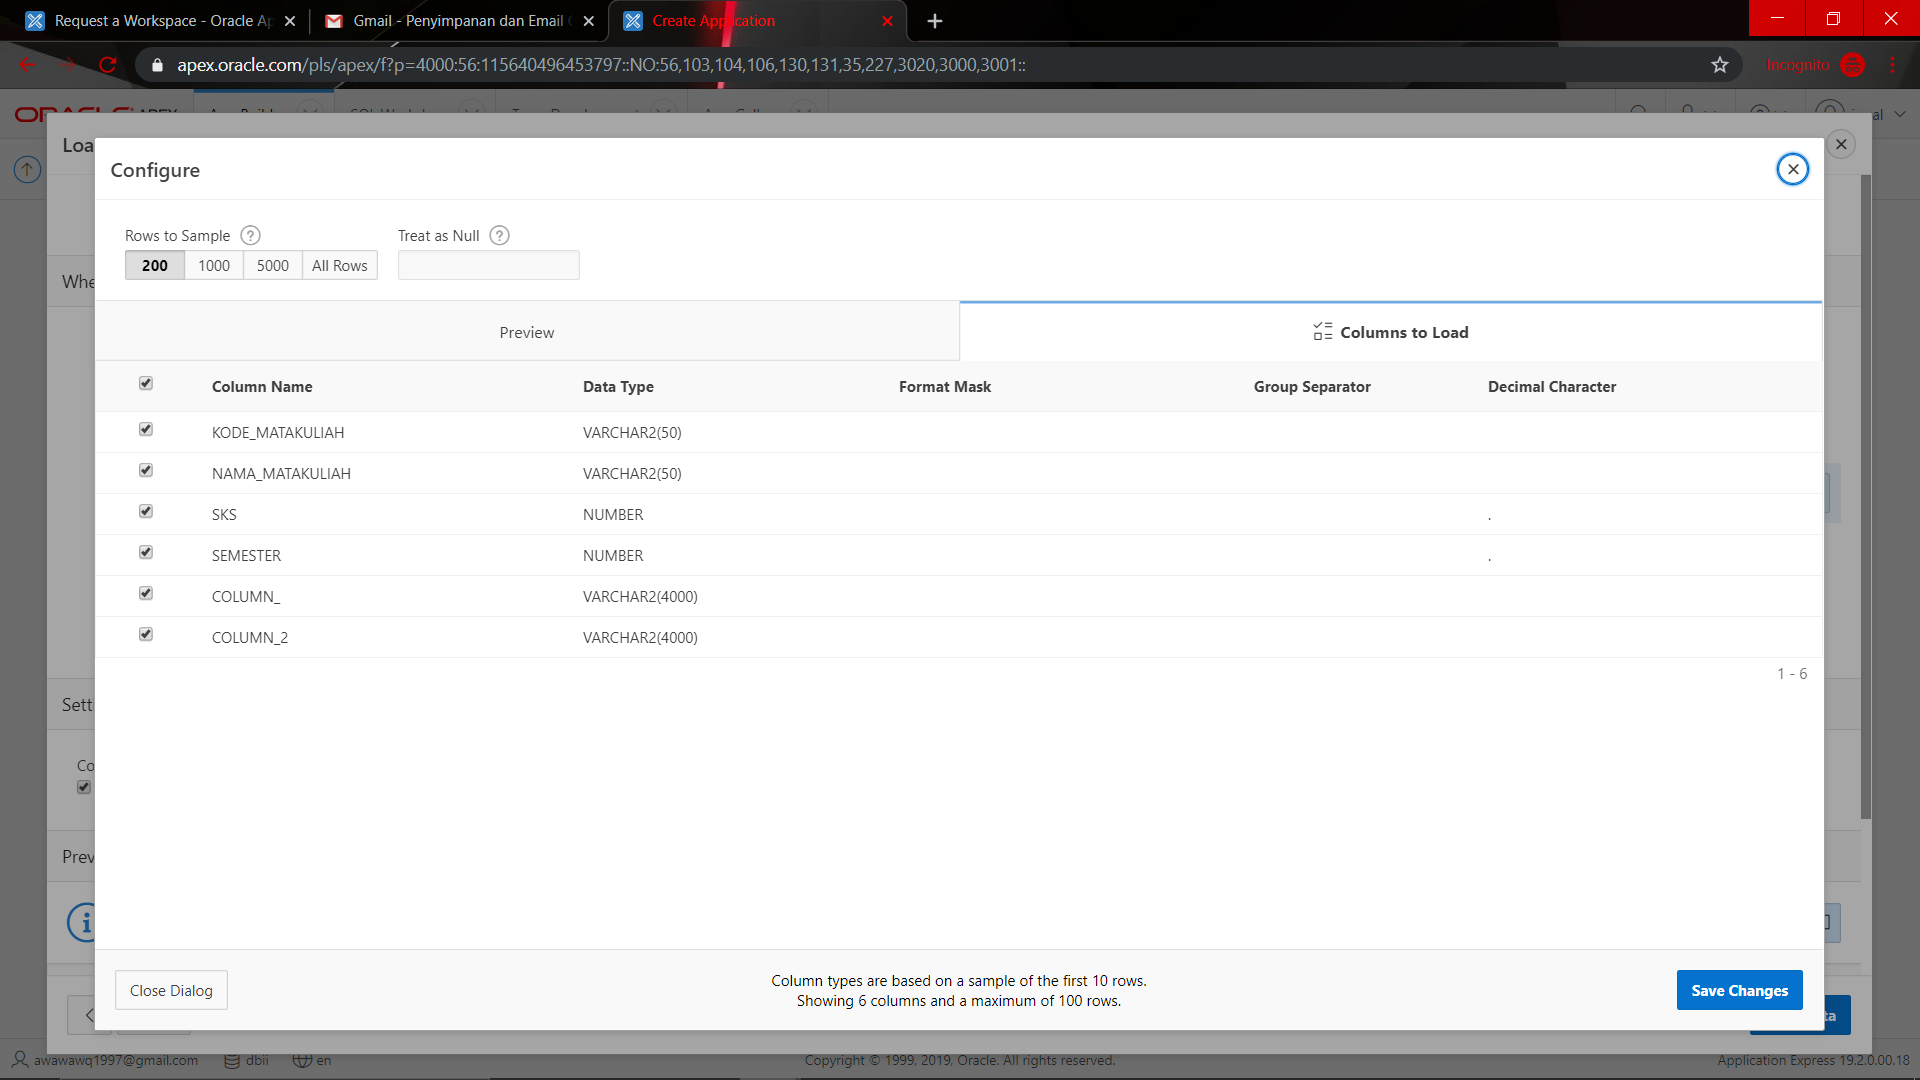
\includegraphics[scale=0.2]{figures/16}
    \caption{Klik error table}
    \label{Environment2}
\end{figure} \\

\item selanjutnya masukan kembali file yang ingin dimasukan 
\begin{figure}[H]
    \centering
    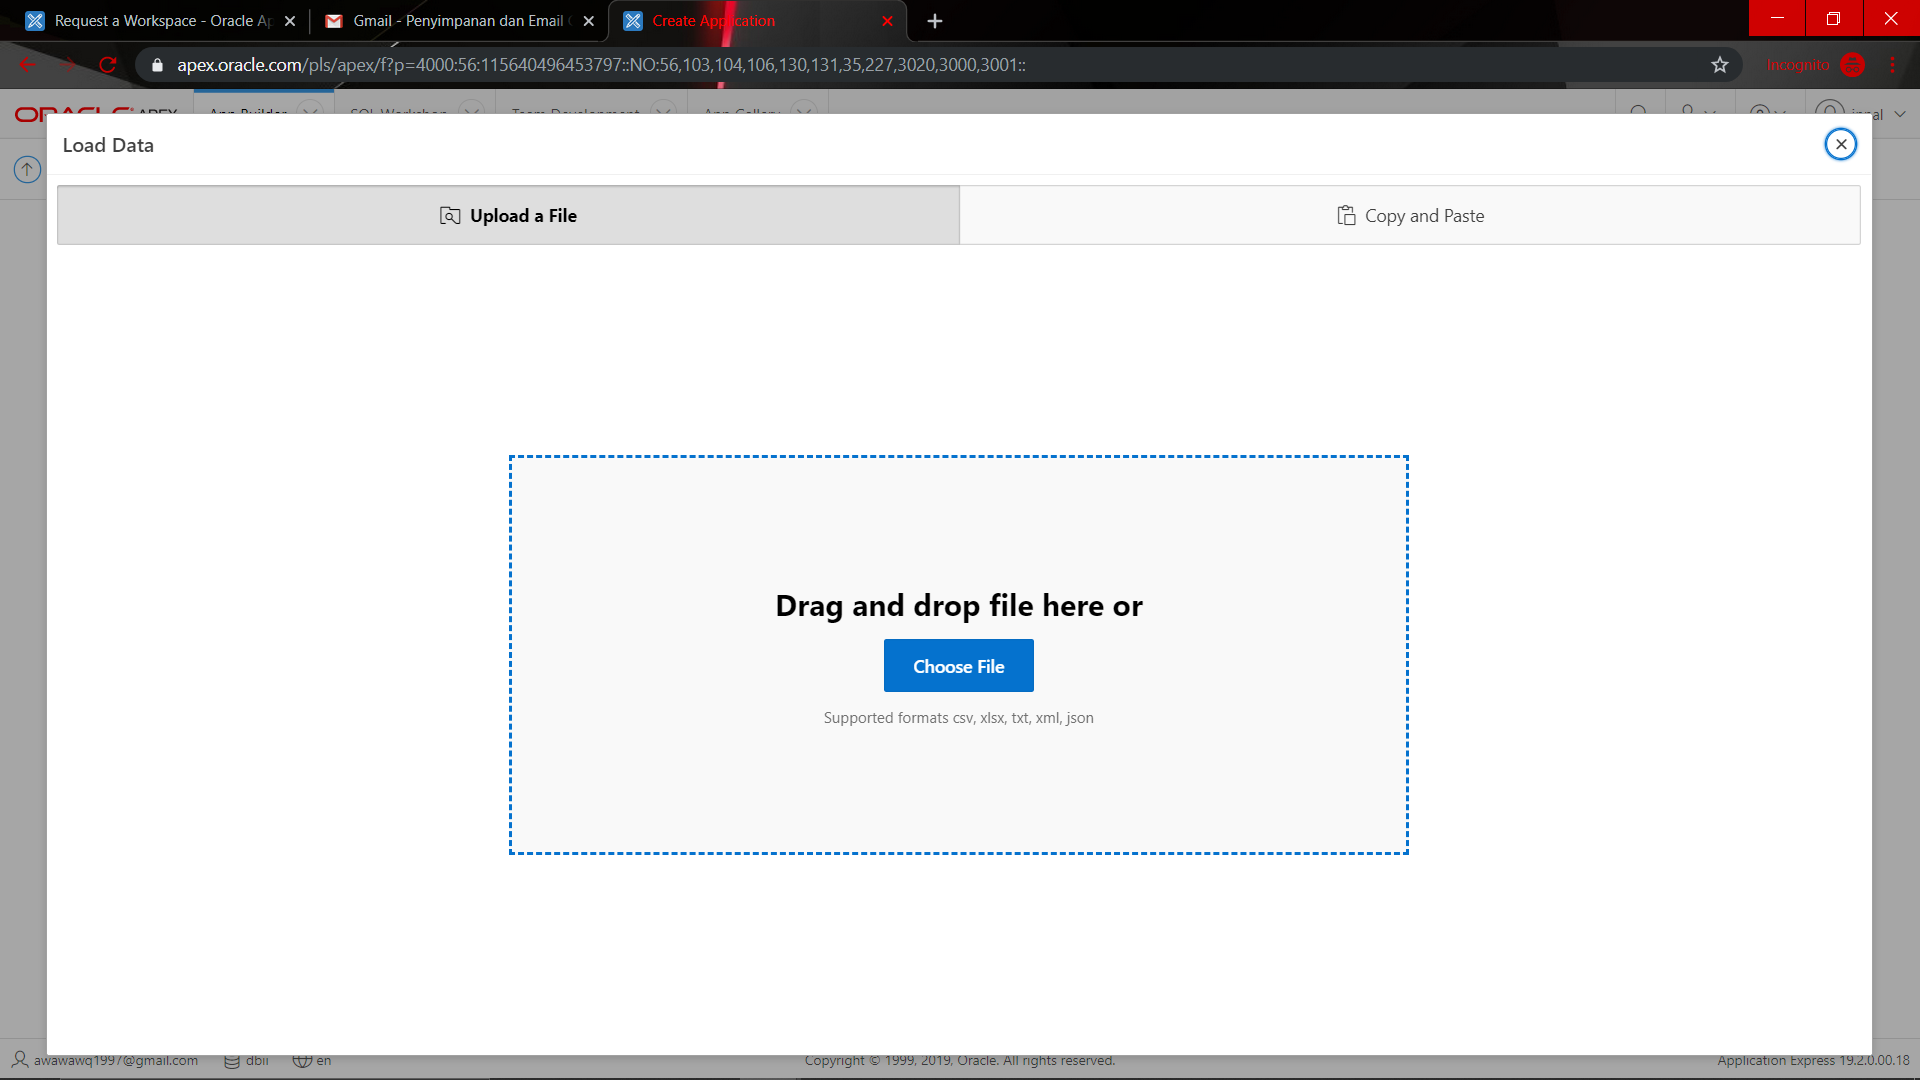
\includegraphics[scale=0.2]{figures/17}
    \caption{Masukan file}
    \label{Environment3}
\end{figure} \\

\item berikan nama untuk file tersebut
\begin{figure}[H]
    \centering
    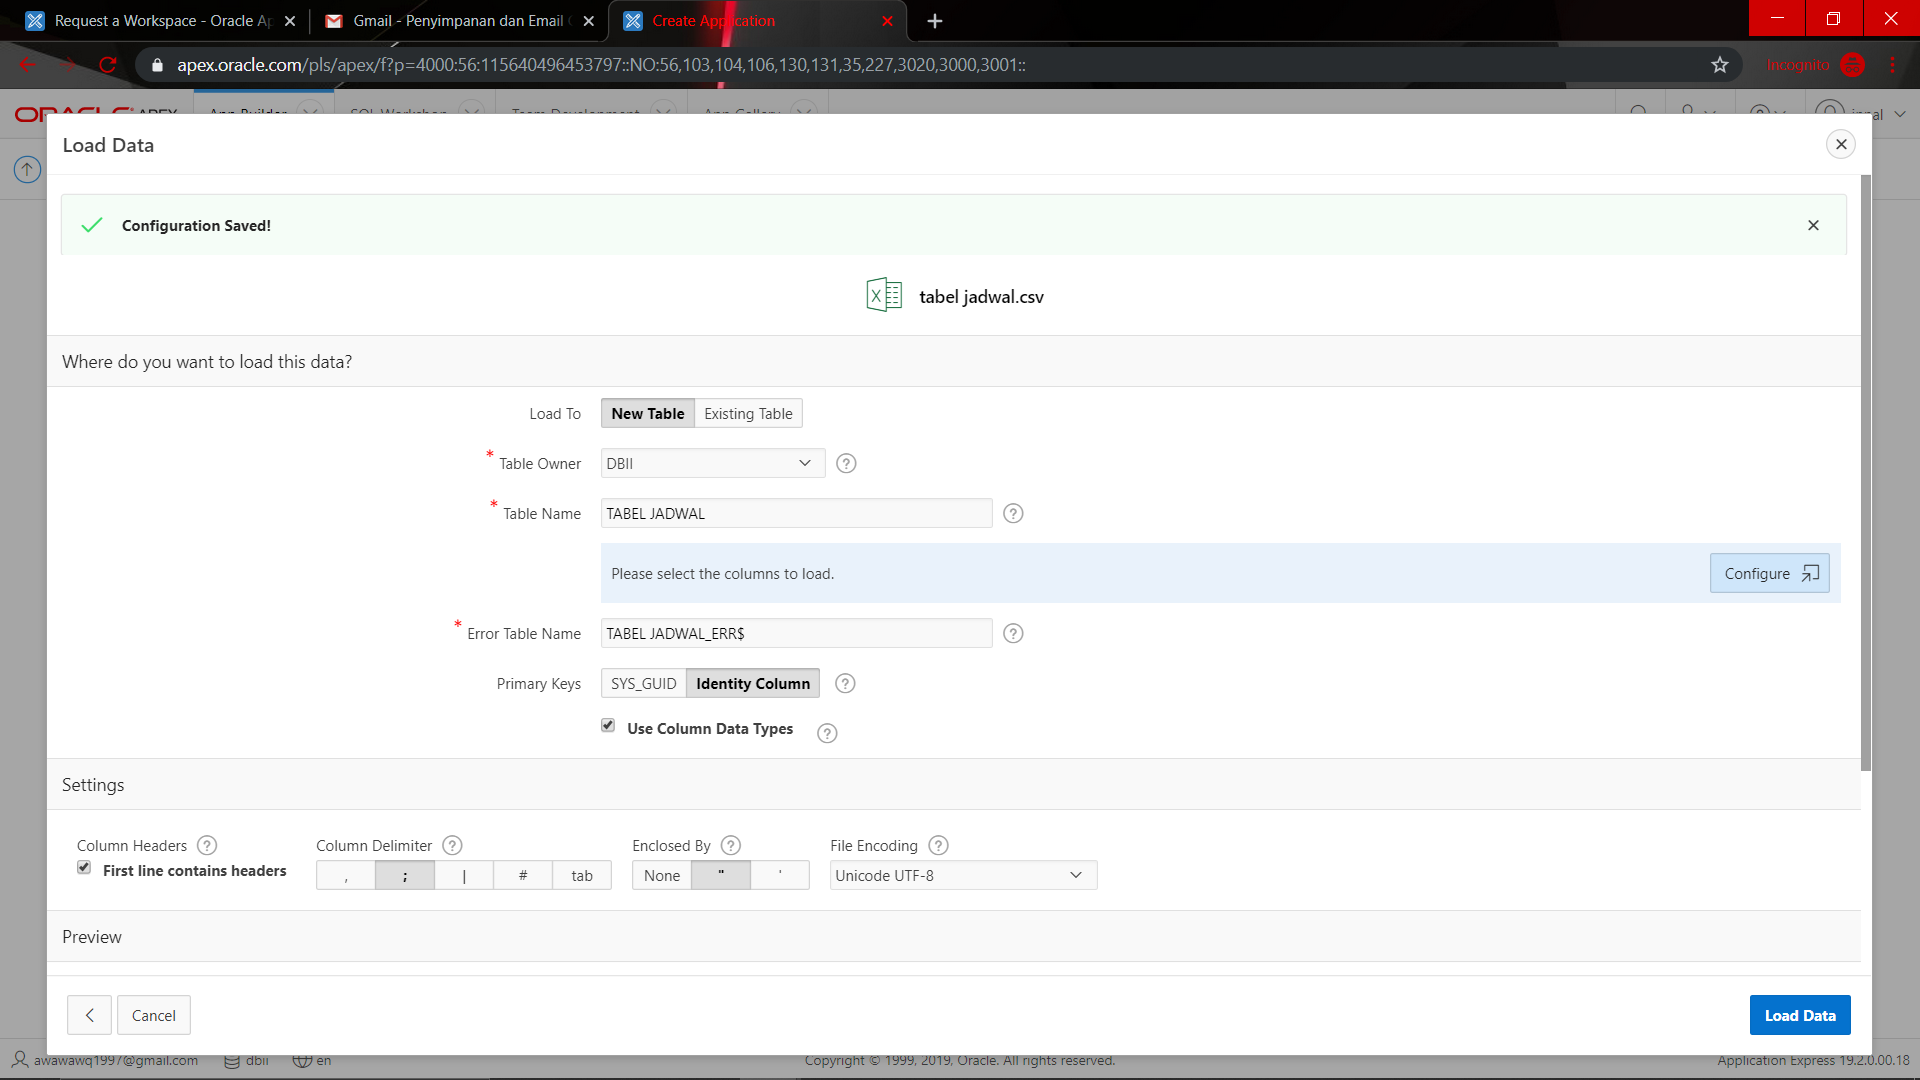
\includegraphics[scale=0.2]{figures/18}
    \caption{Berikan nama}
    \label{Environment4}
\end{figure} \\

\item lalu klik create application
\begin{figure}[H]
    \centering
    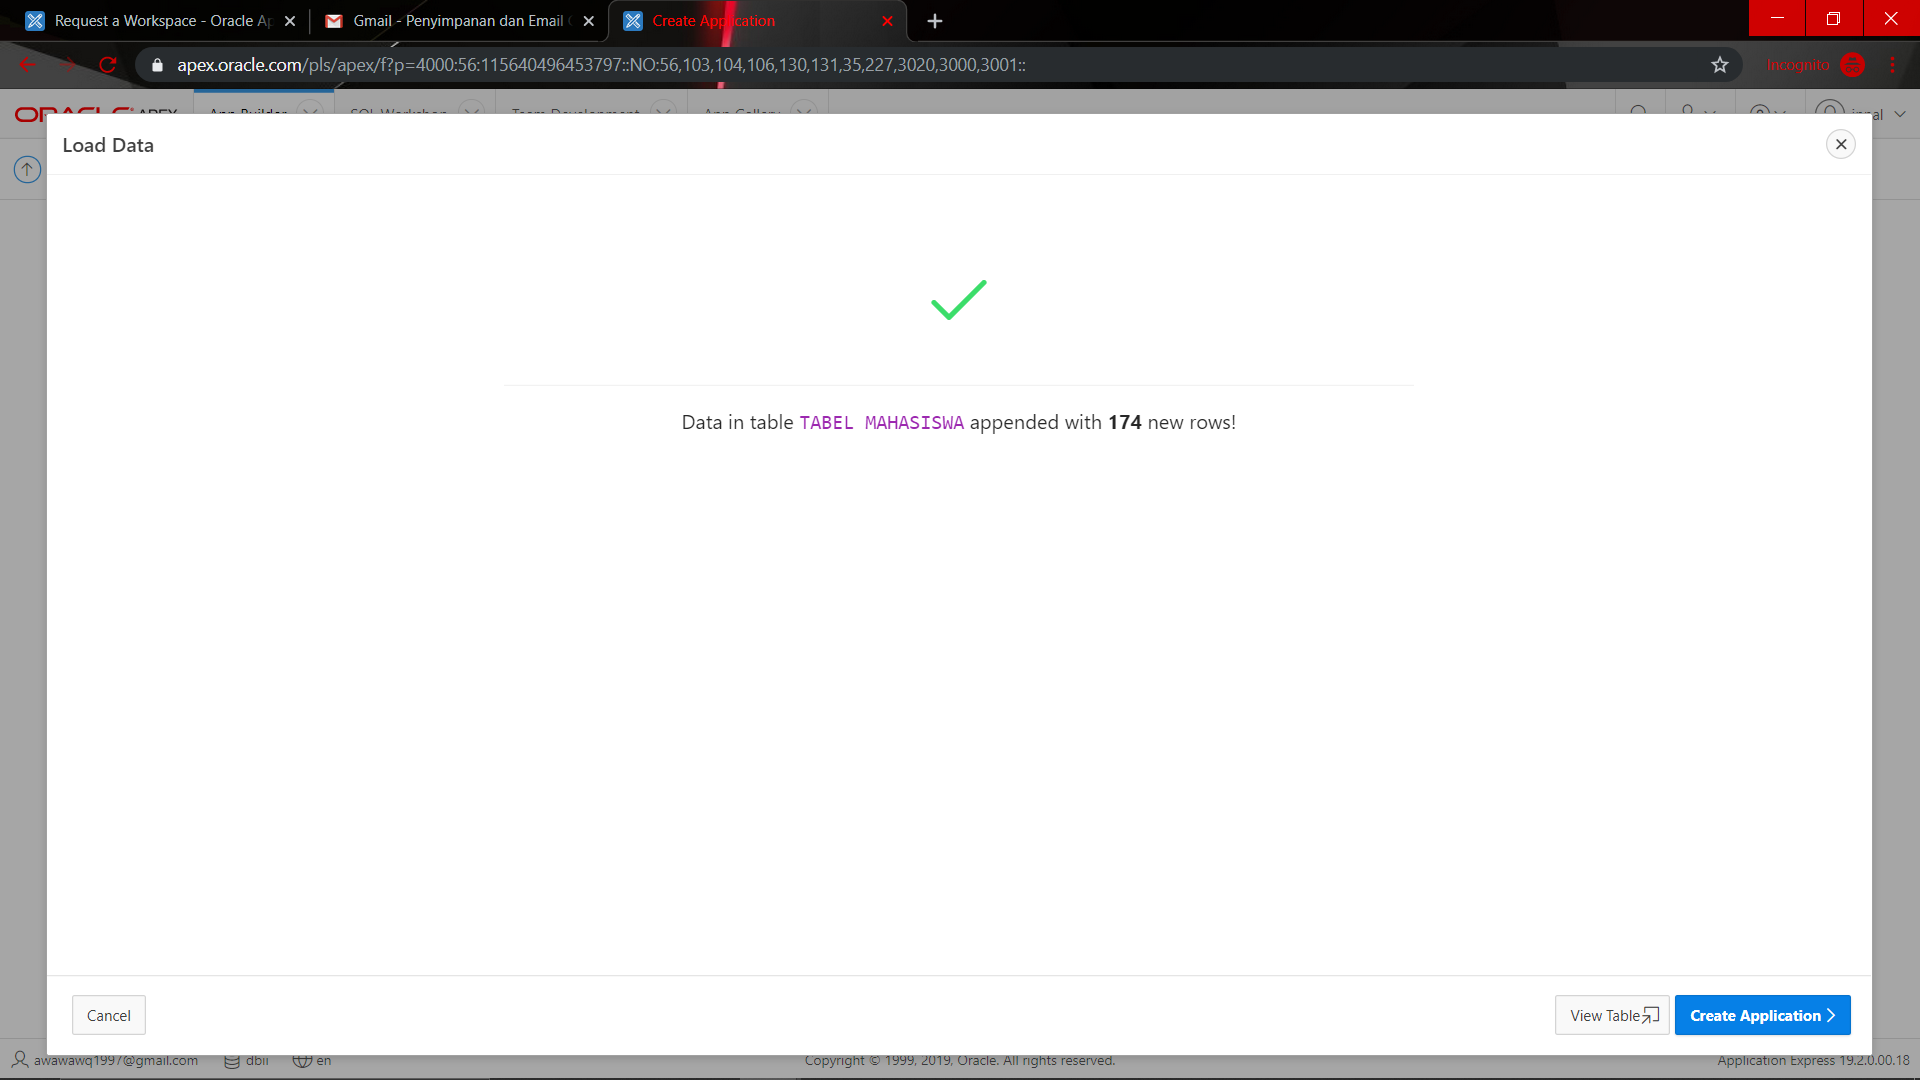
\includegraphics[scale=0.2]{figures/19}
    \caption{Creat aplication}
    \label{Environment5}
\end{figure} \\

\item setelah itu klik add page 
\begin{figure}[H]
    \centering
    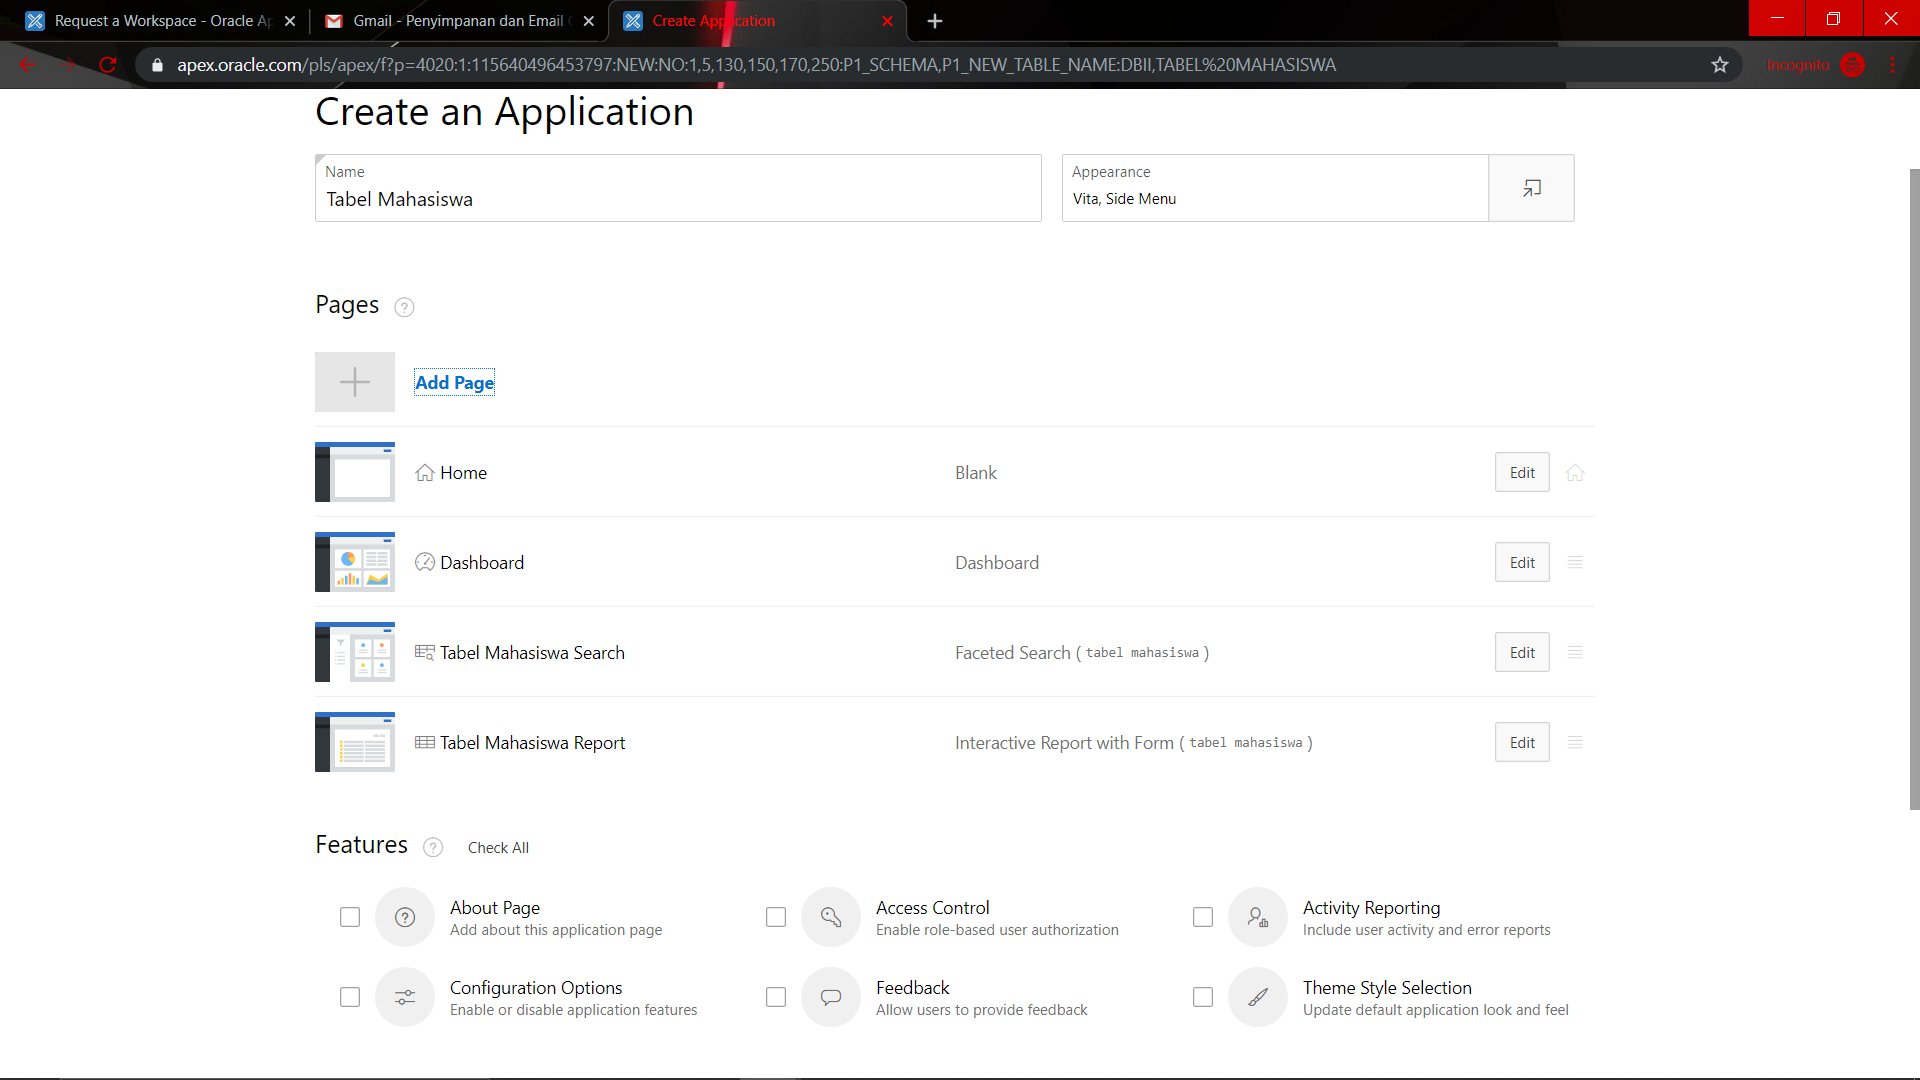
\includegraphics[scale=0.2]{figures/20}
    \caption{Add page}
    \label{CLI}
\end{figure} \\


\item klik interactive report
\begin{figure}[H]
    \centering
    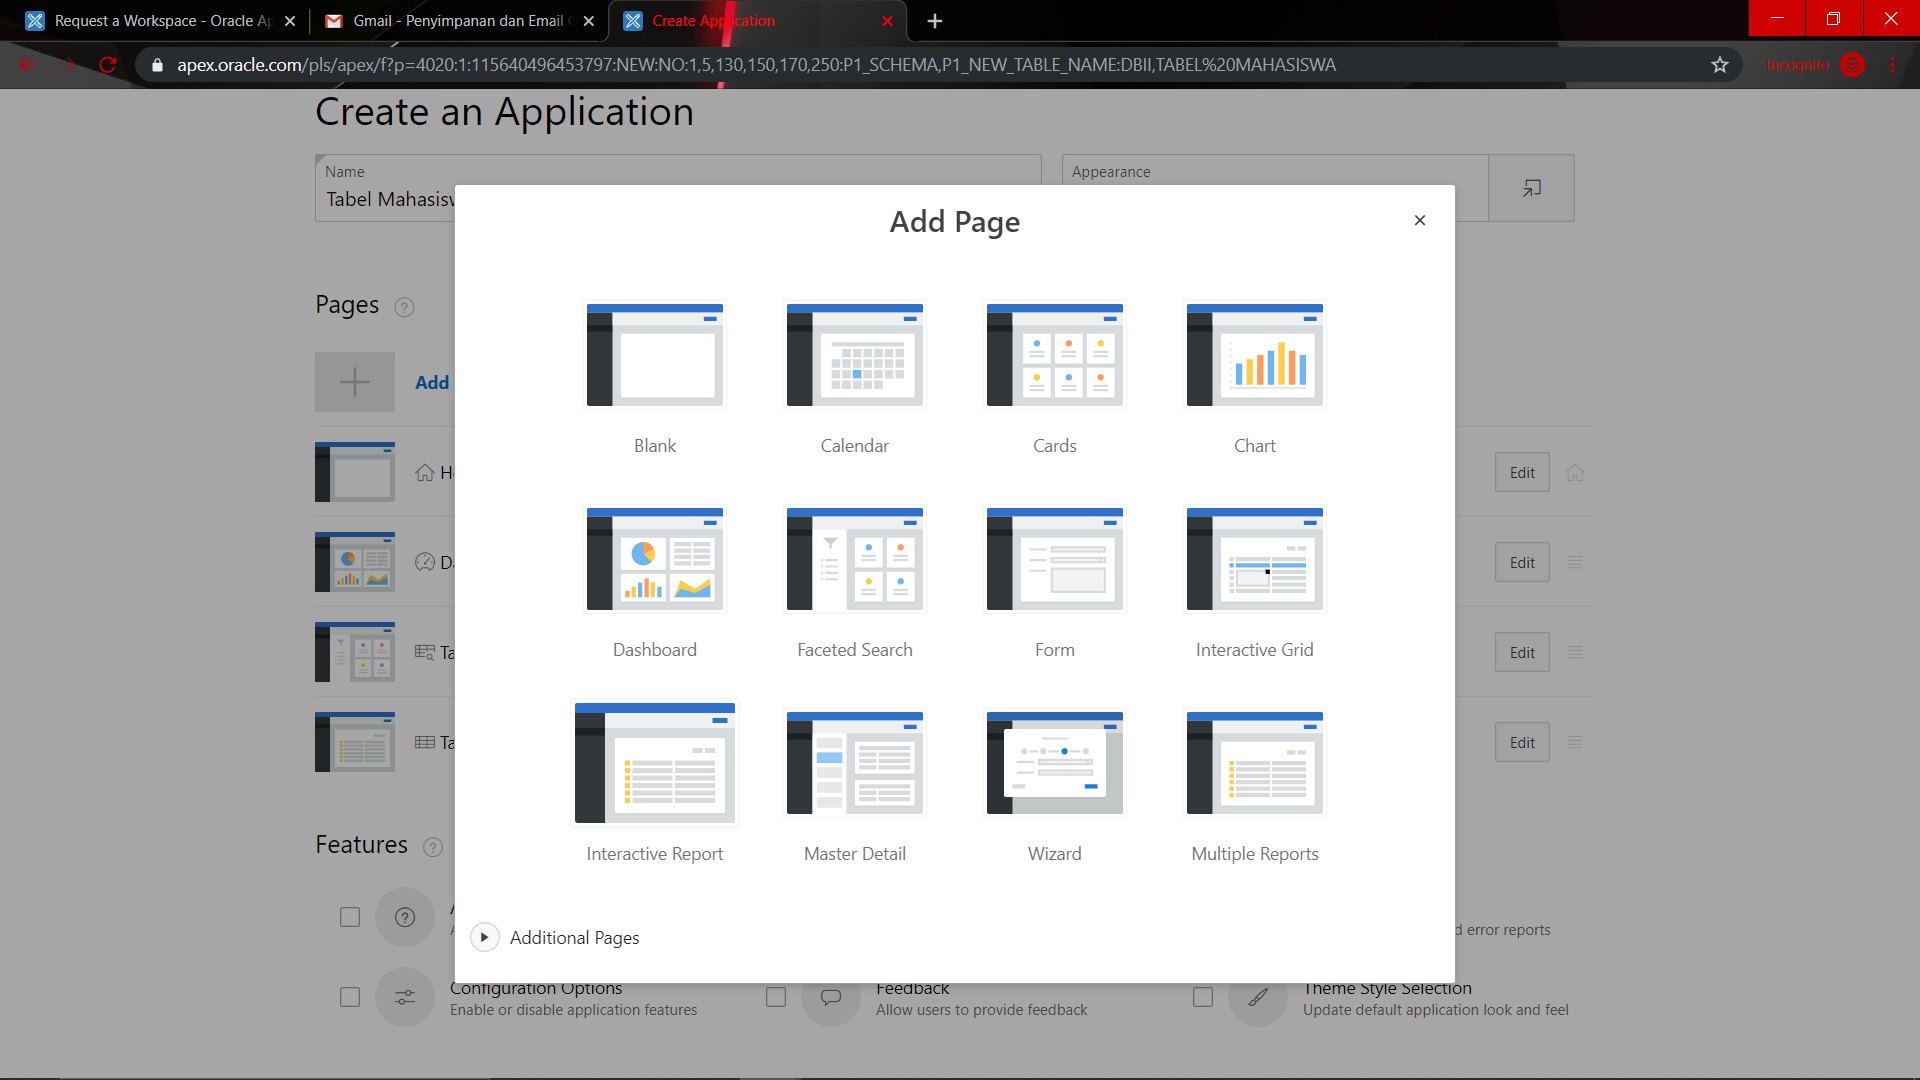
\includegraphics[scale=0.2]{figures/21}
    \caption{klik interactive report}
    \label{Anaconda Navigator}
\end{figure} \\

\item berikan nama page tersebut klik table or view dan klik table yang ingin di masukan ke page itu.
\begin{figure}[H]
    \centering
    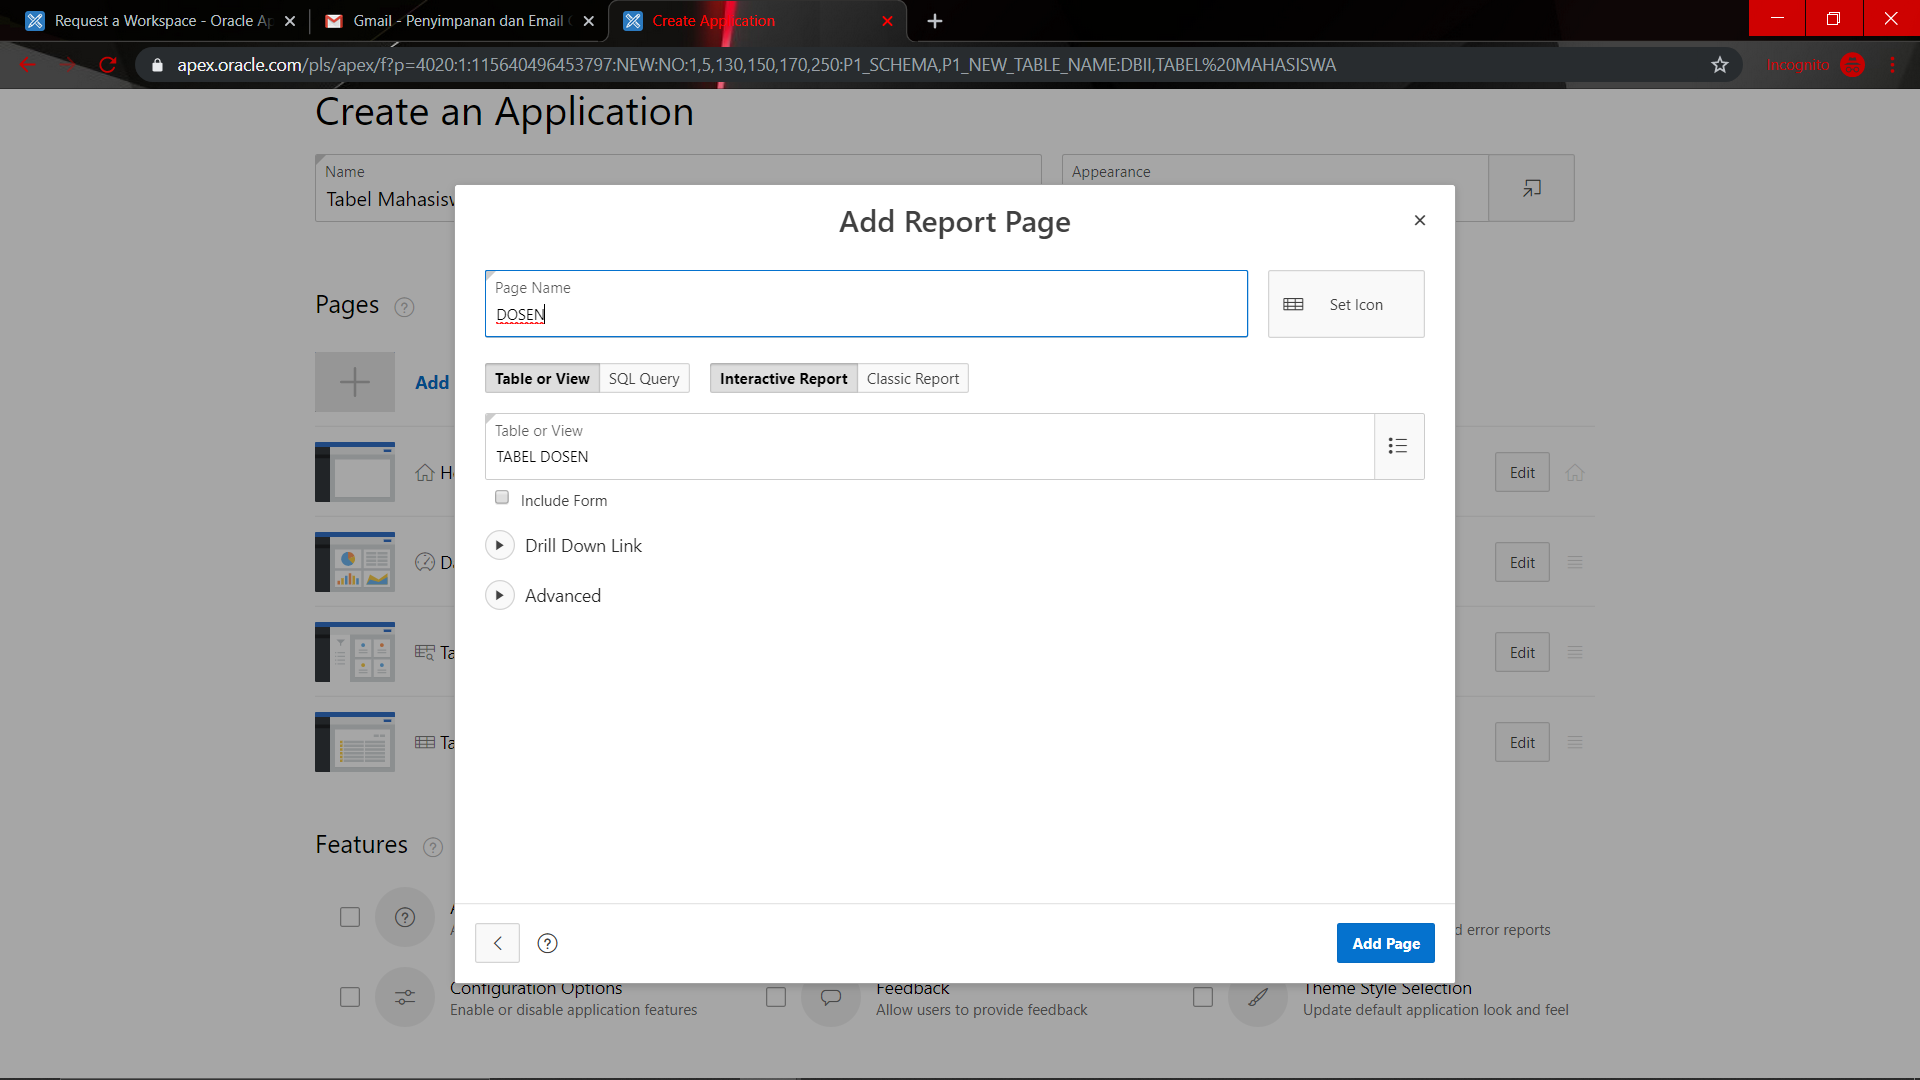
\includegraphics[scale=0.2]{figures/22}
    \caption{Berikan nama}
    \label{Print Hello World}
\end{figure} \\

\item lakukan hal yang sama seperti sebelumnya tetapi pilih table yang lain yang ingin di masukan
\begin{figure}[H]
    \centering
    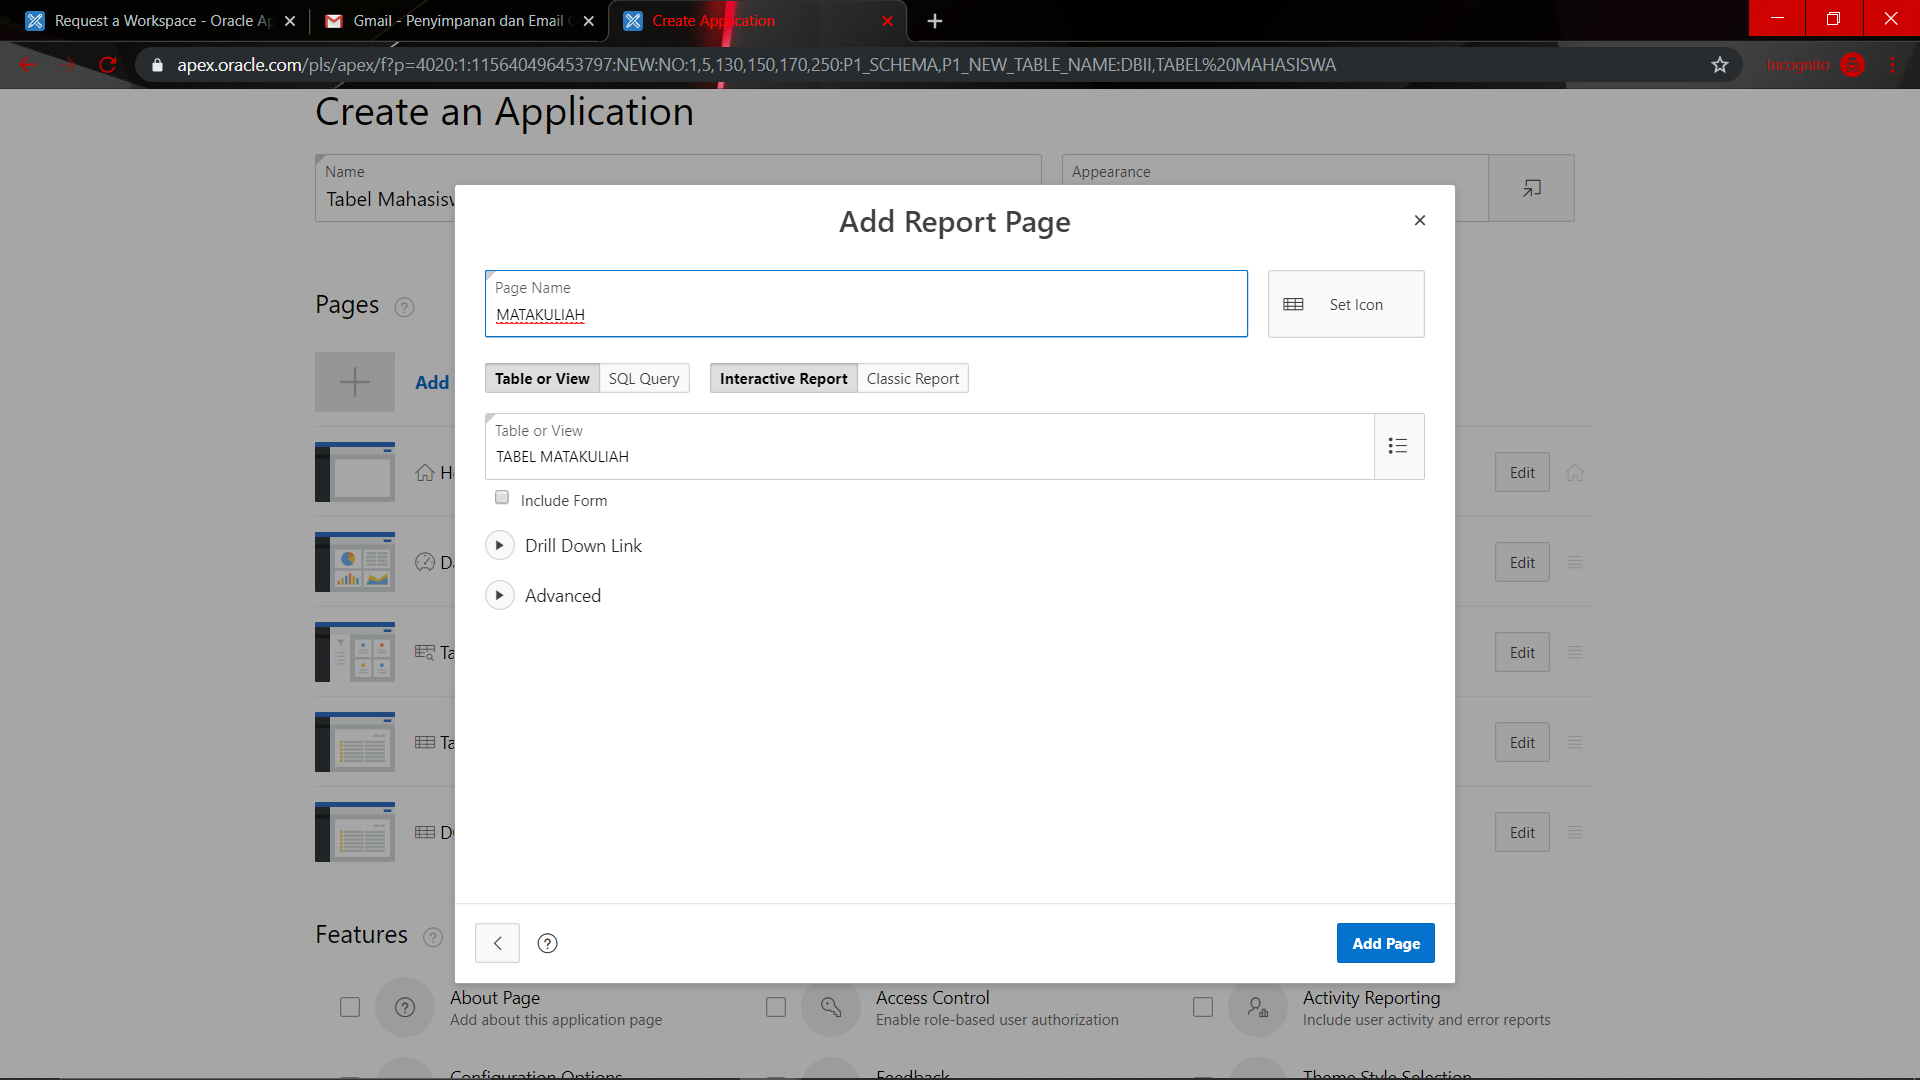
\includegraphics[scale=0.2]{figures/23}
    \caption{Masukan kembali table}
    \label{Hello World}
\end{figure} \\

\item lakukan hal yang sama seperti sebelumnya tetapi pilih table yang lain yang ingin di masukan
\begin{figure}[H]
    \centering
    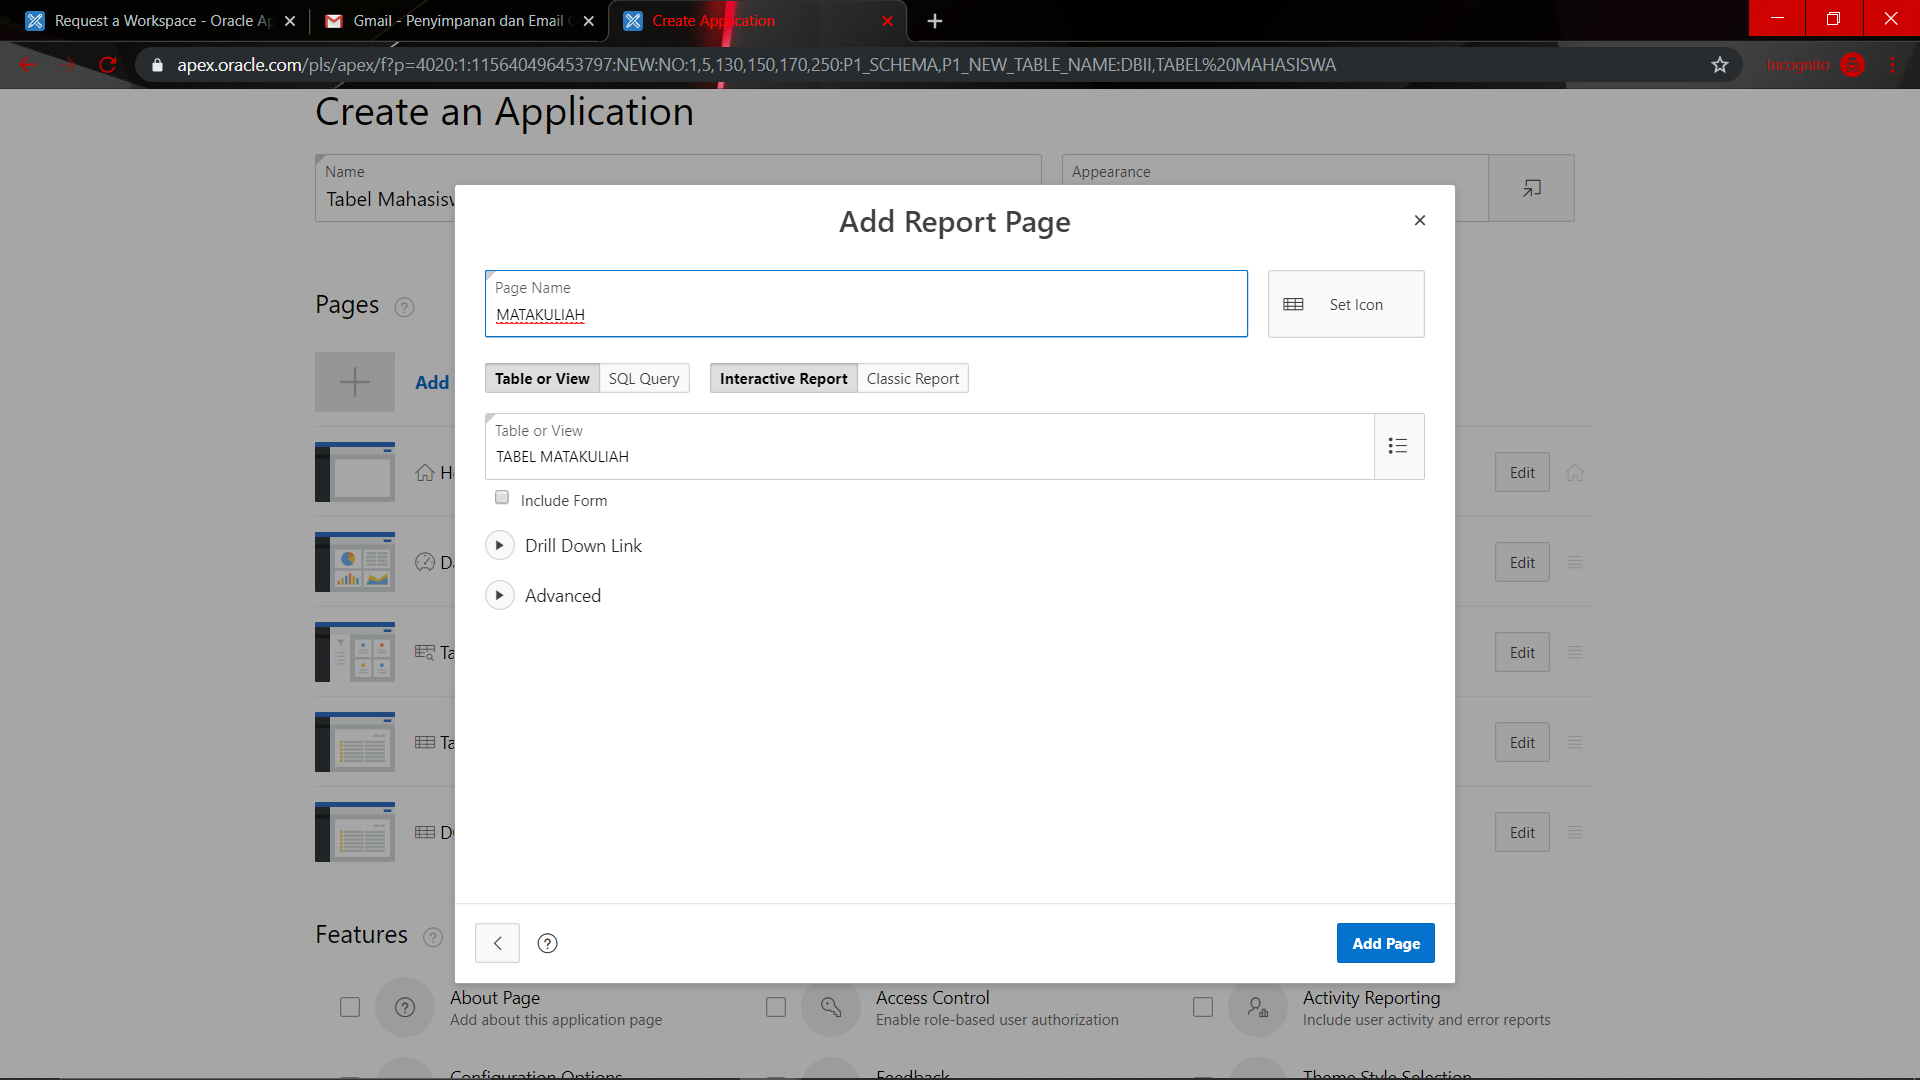
\includegraphics[scale=0.2]{figures/23}
    \caption{Masukan kembali}
    \label{Automatic1}
\end{figure} \\

\item lakukan hal yang sama seperti sebelumnya tetapi pilih table yang lain yang ingin di masukan
\begin{figure}[H]
    \centering
    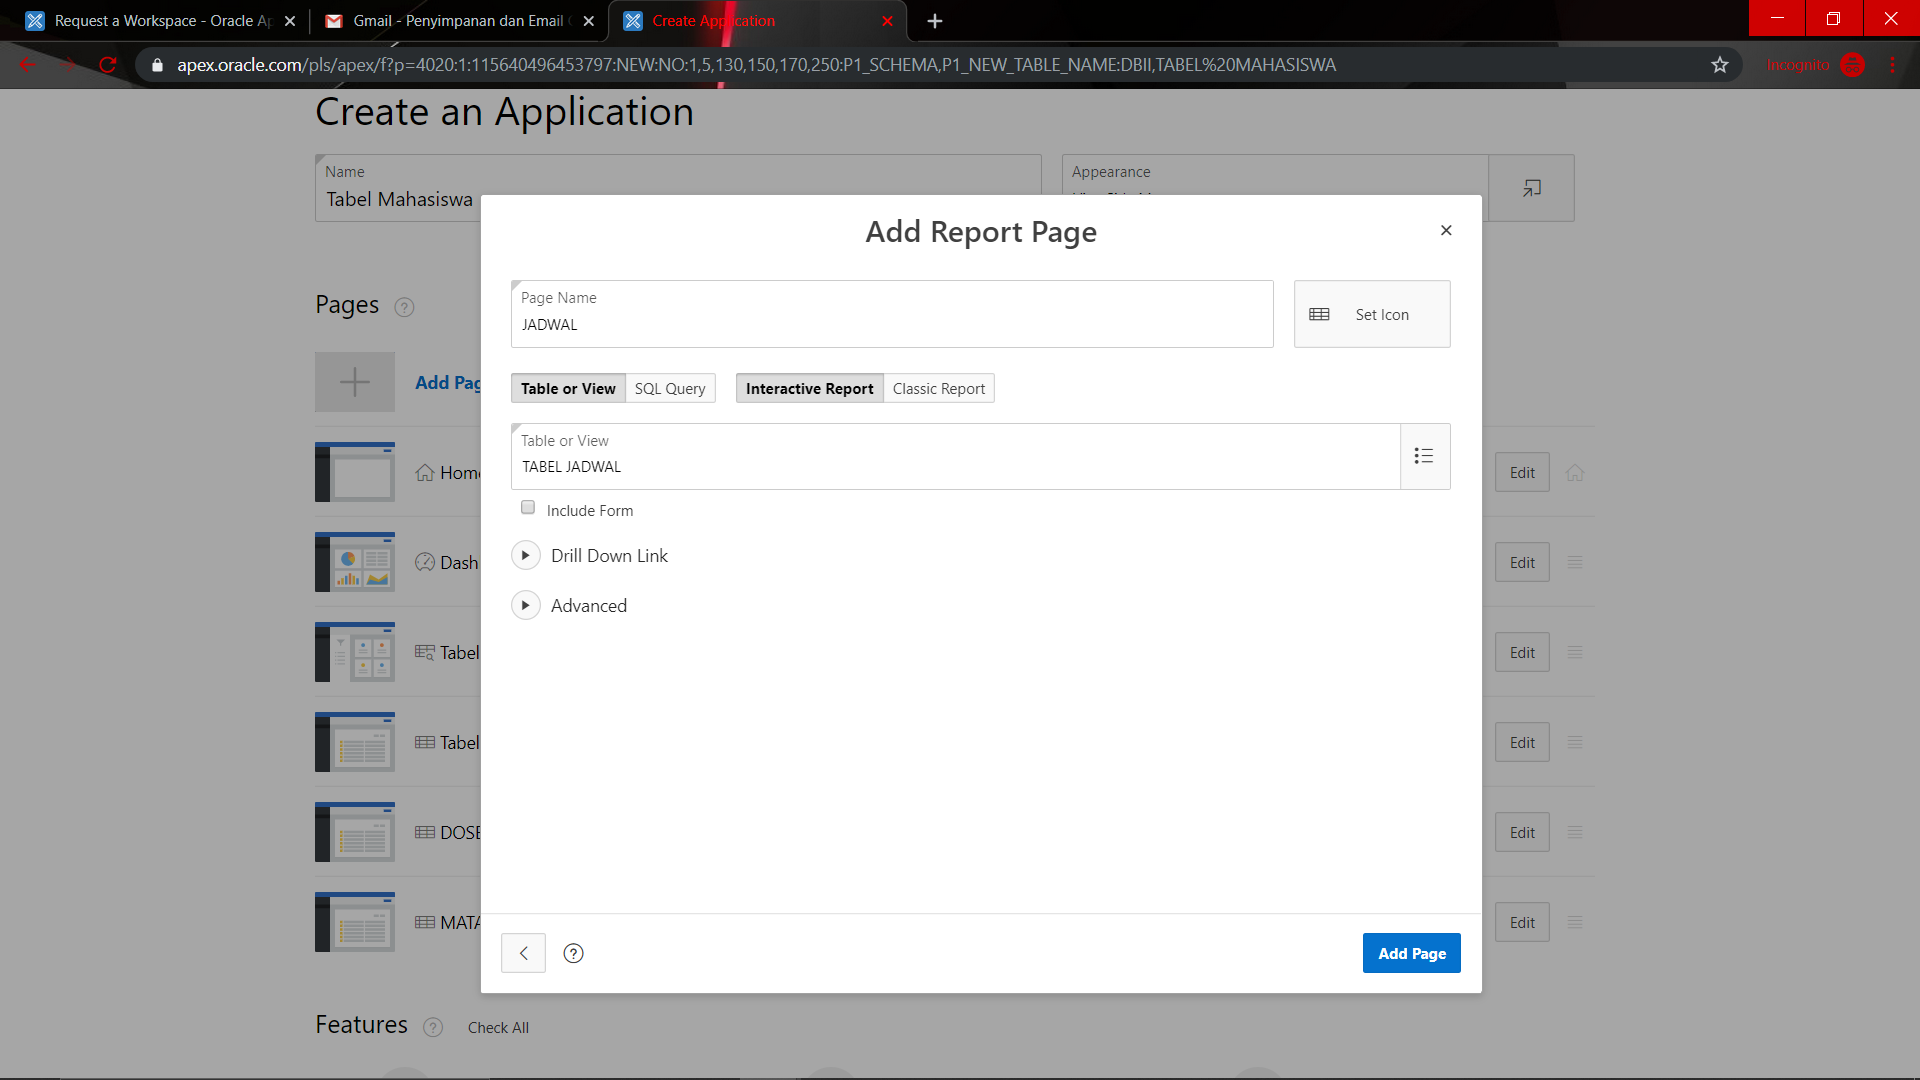
\includegraphics[scale=0.2]{figures/24}
    \caption{Masukan kembali}
    \label{Automatic2}
\end{figure} \\

\item lakukan hal yang sama seperti sebelumnya tetapi pilih table yang lain yang ingin di masukan
\begin{figure}[H]
    \centering
    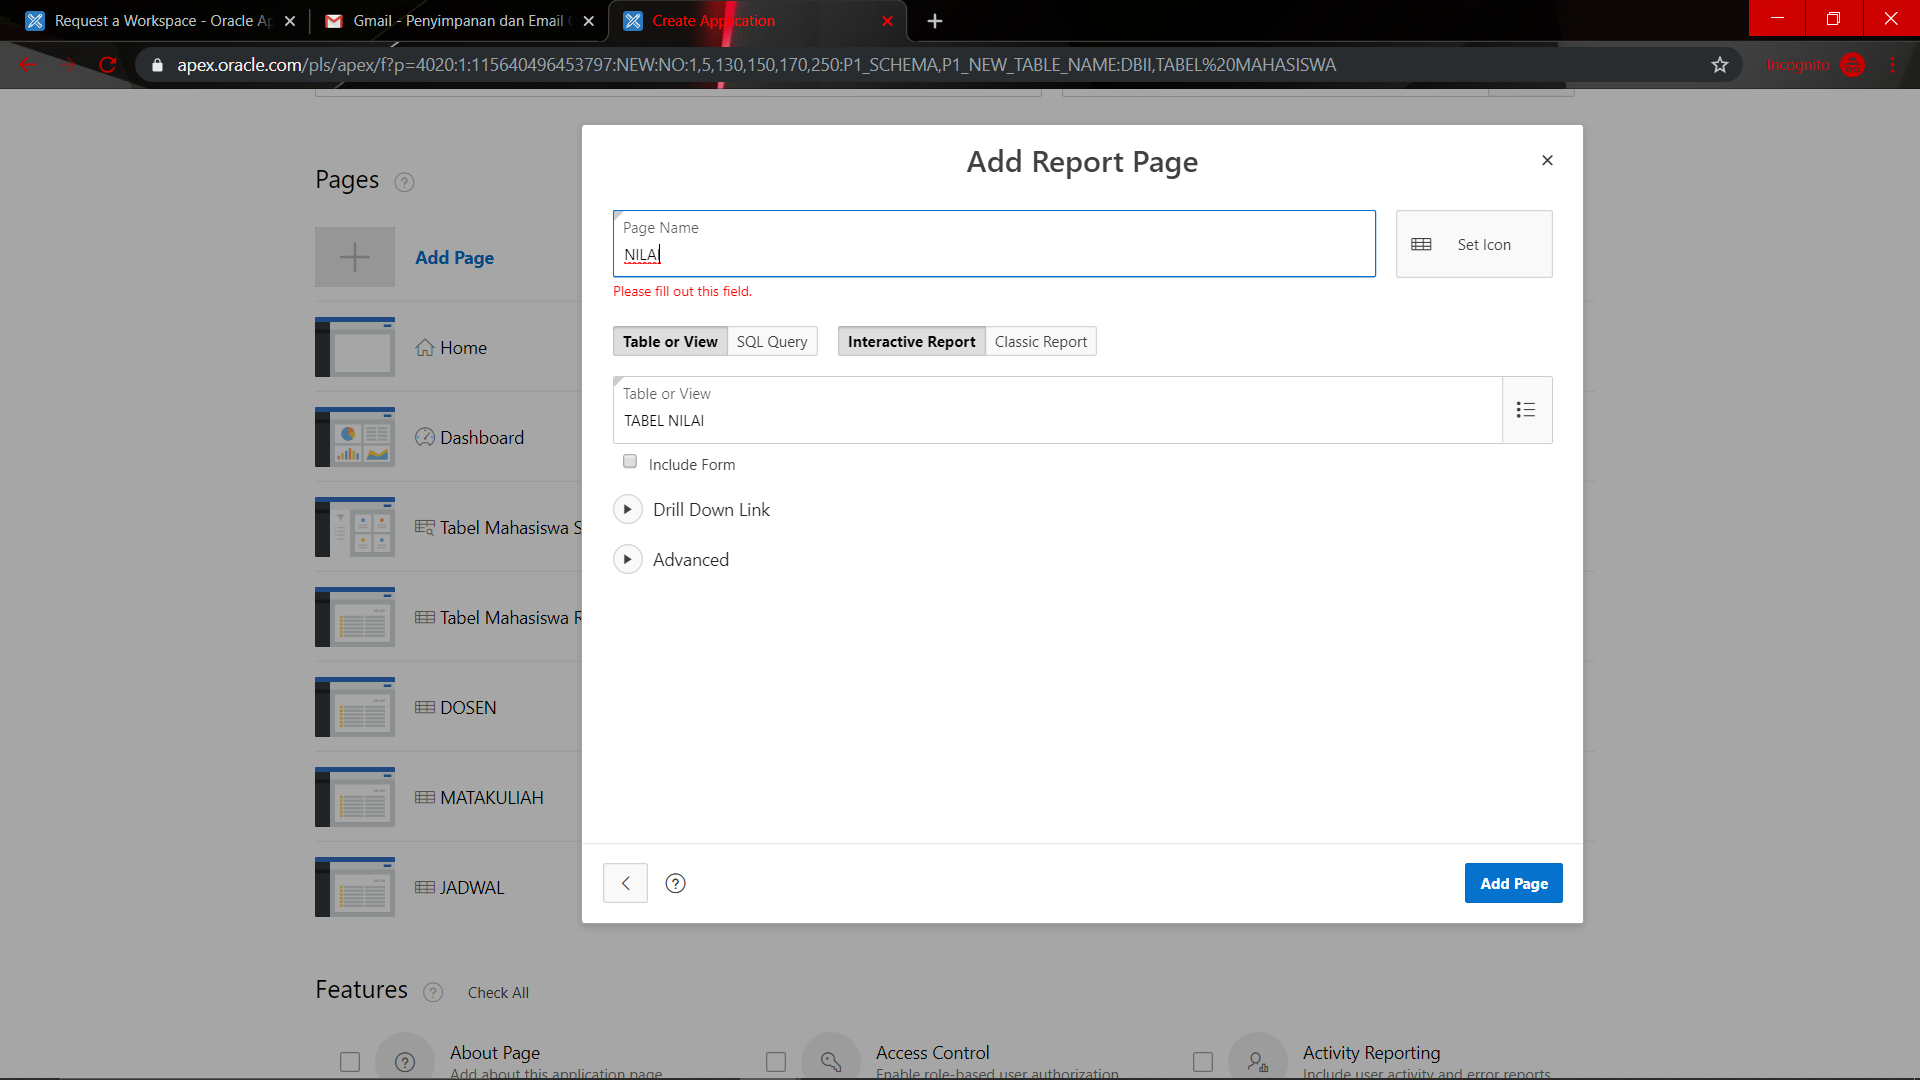
\includegraphics[scale=0.2]{figures/25}
    \caption{Masukan kembali}
    \label{Automatic3}
\end{figure} \\

\item Kemudian pilih add page lagi,isikan page name ”NILAI” lalu klik SQL query dan ketiklah pada SQL query seperti dibawah ini. kemudian klik add page \\

\item setelah memasukan semua table ke page klik create application
\begin{figure}[H]
    \centering
    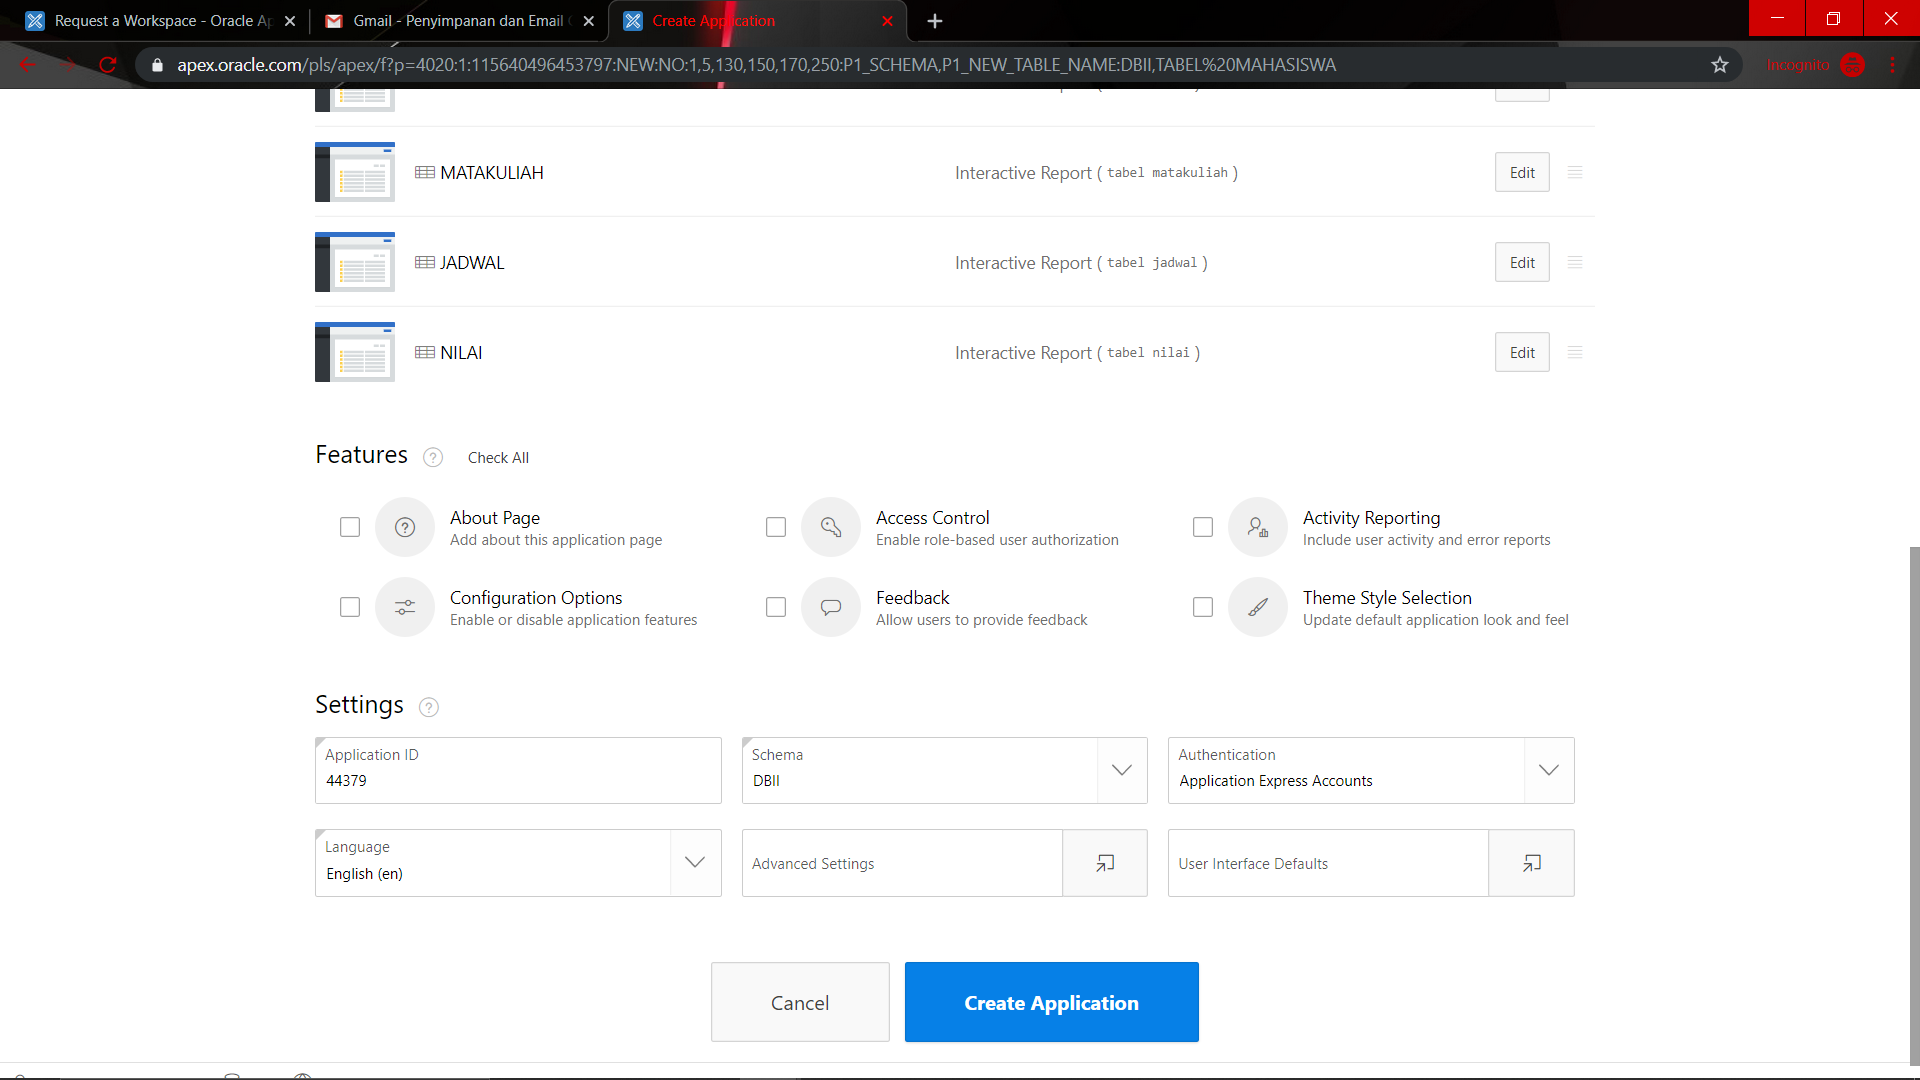
\includegraphics[scale=0.2]{figures/26}
    \caption{ Masukan kembali semua table ke page }
    \label{Automatic4}
\end{figure} \\

\item masukan username dan password
\begin{figure}[H]
    \centering
    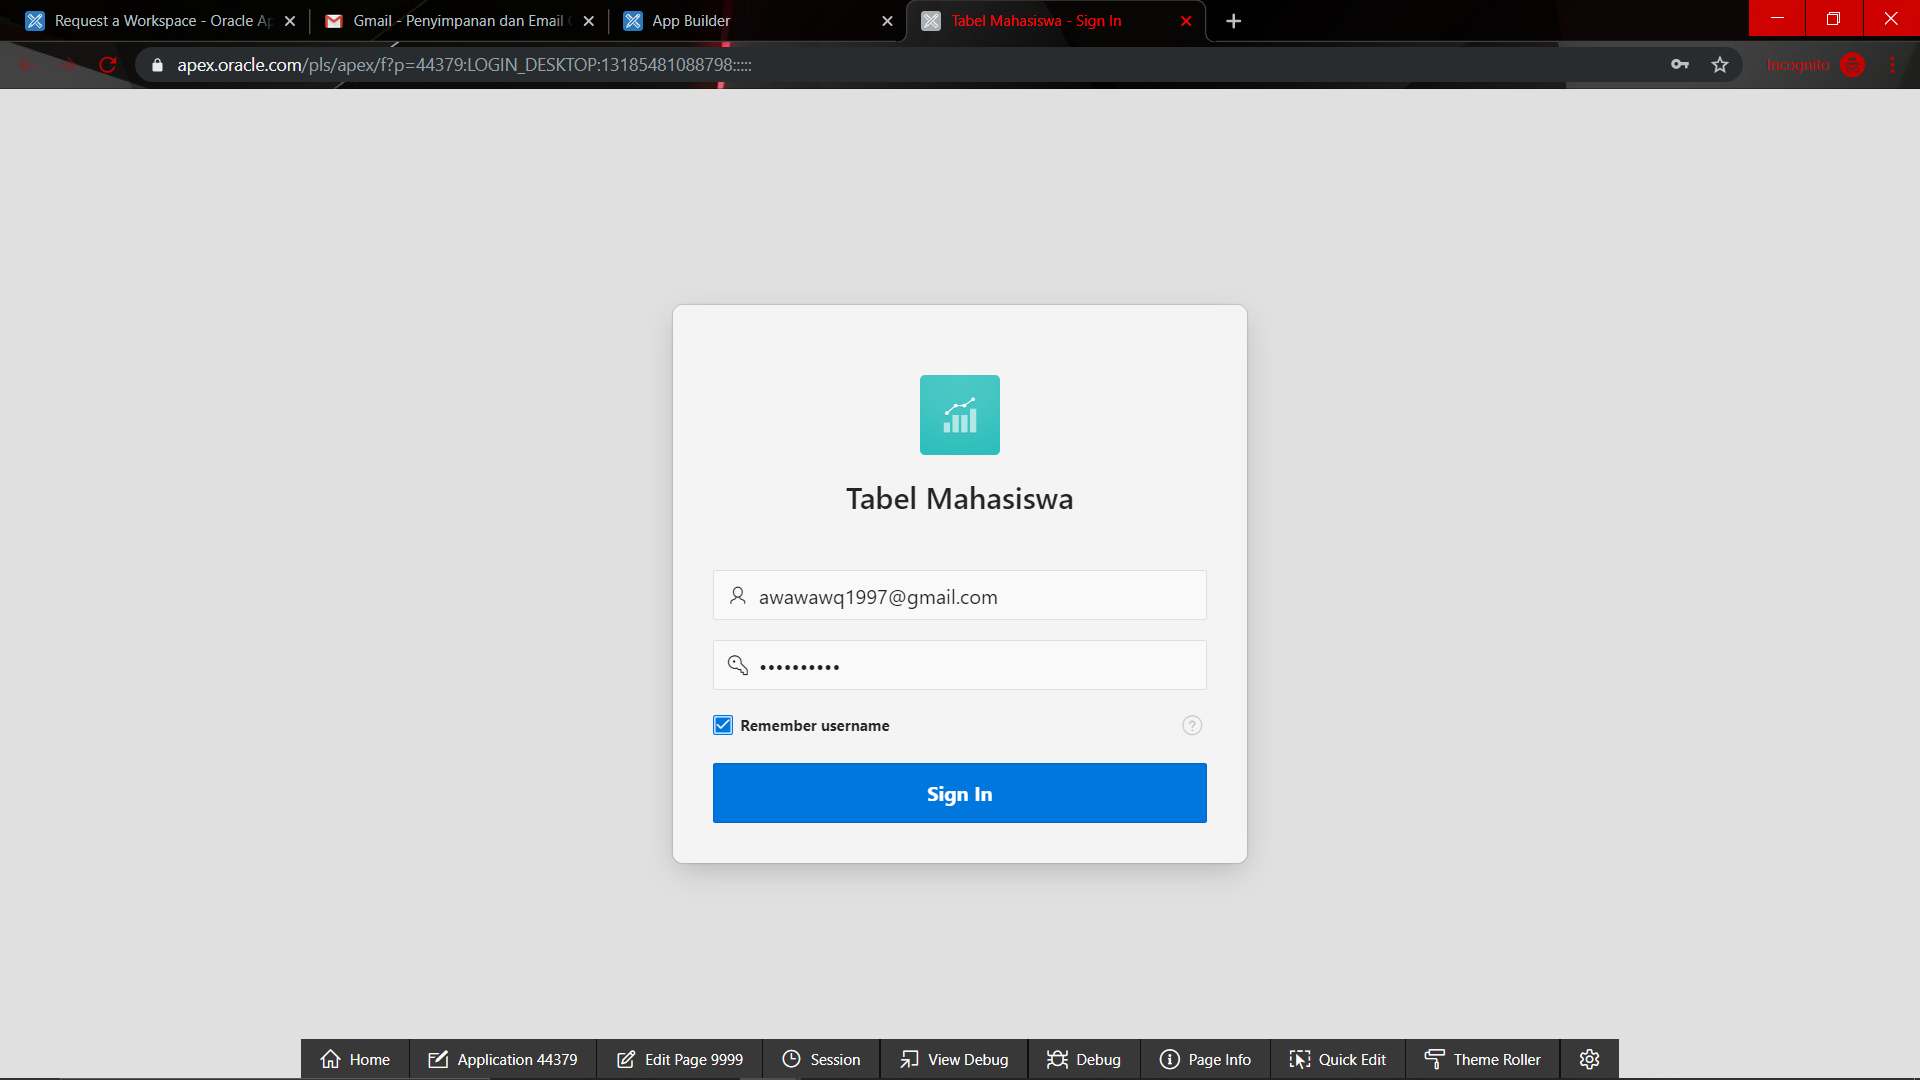
\includegraphics[scale=0.2]{figures/27}
    \caption{ masukan kembali username dan password}
    \label{Variable Explorer}
\end{figure} \\

\item aplikasi apex telah selesai dibuat
\begin{figure}[H]
    \centering
    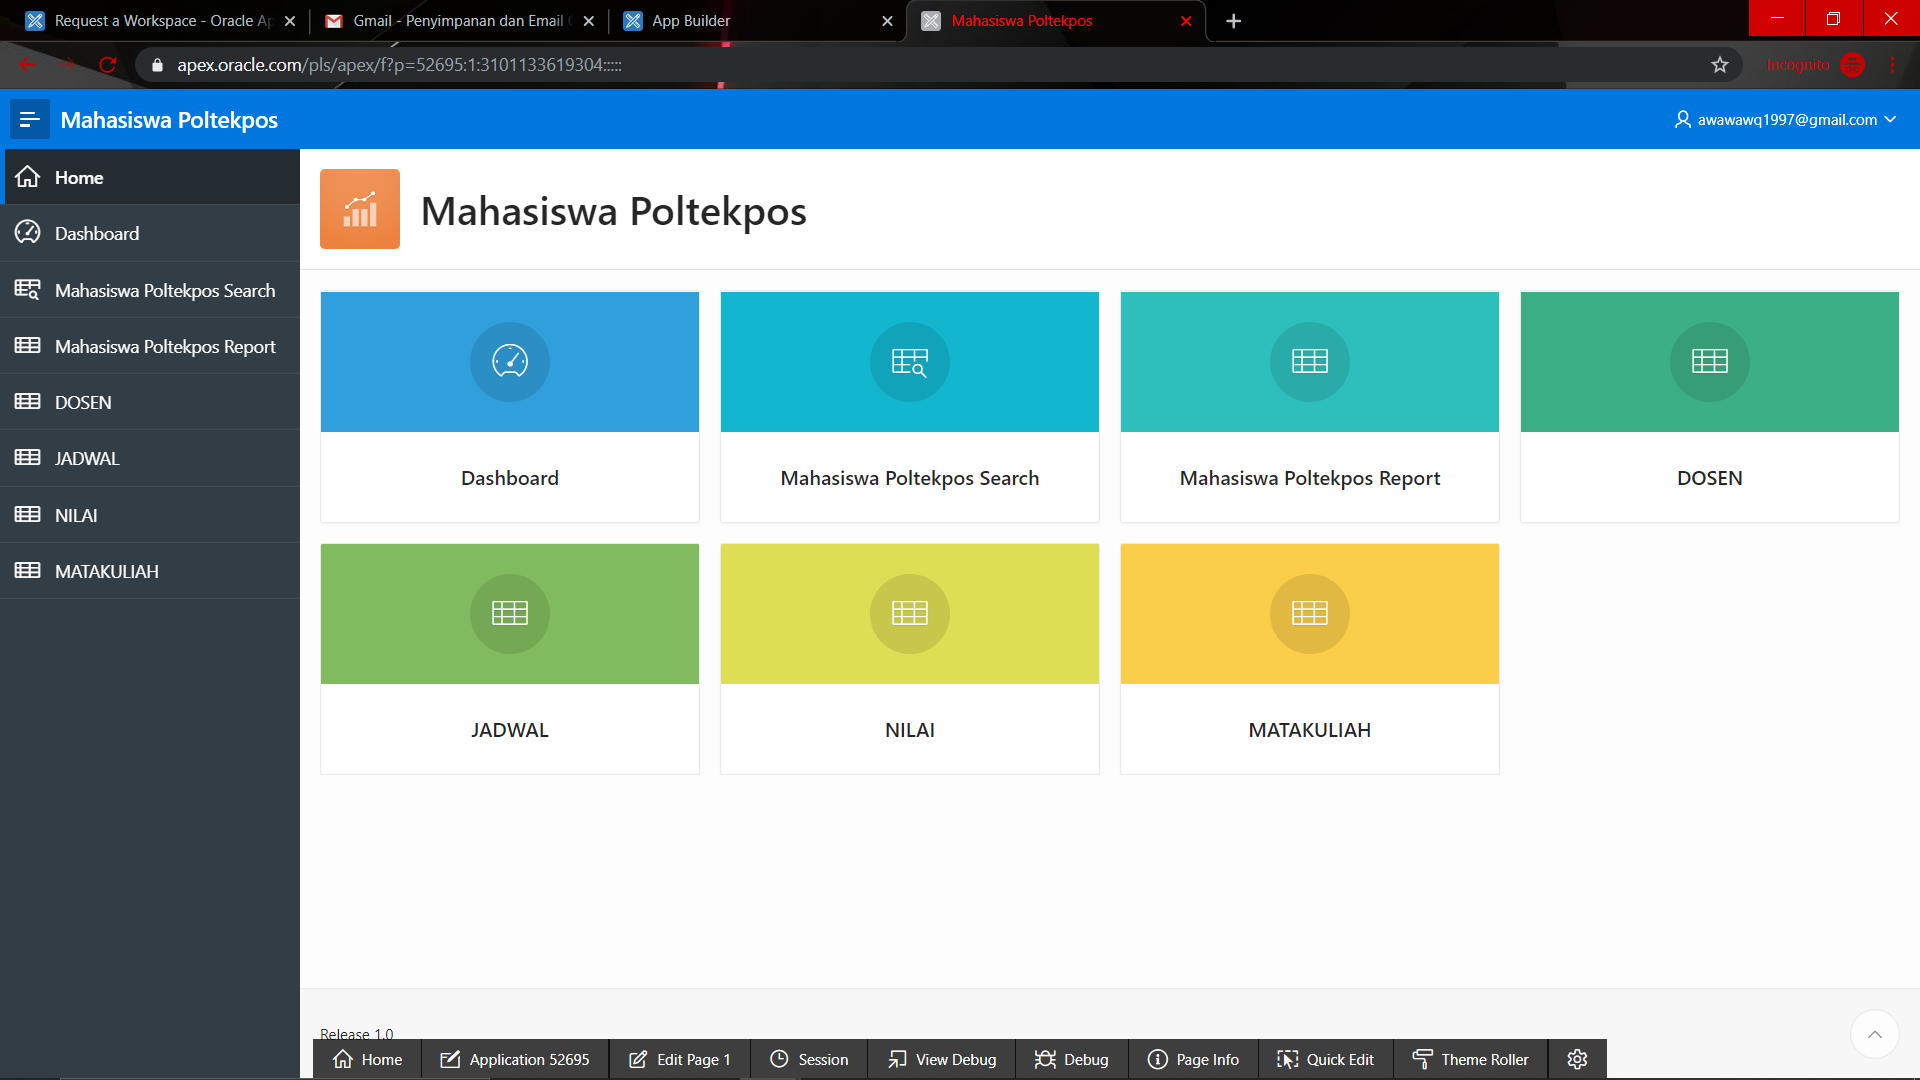
\includegraphics[scale=0.2]{figures/28}
    \caption{ Aplikasi selesai dibuat}
    \label{Indentasi}
\end{figure}
\end{enumerate}

\par 
Username : cecepgunawan48@gmail.com \\
Password : Homeswethome48! \\
Workspace :proyekii \\
link     : https://apex.oracle.com/pls/apex/f?p=52695:1:35108638267405:::::
